\chapter{Marco Teórico}
	\section{Mantenimiento}
		\subsection{Generalidades del mantenimiento}
			El mantenimiento en la industria es simplemente la acción de mantener a una máquina ejerciendo de manera correcta la función para la cual fue construida. El origen de la mantención viene ligada con el origen de las herramientas, el simple hecho de afilar un cuchillo puede considerarse mantenimiento. Sin embargo, con la llegada de la revolución industrial y los procesos productivos (ej. Ford y la producción en serie con la llegada de máquinas cada vez más complejas y especificas en su función), es que se el mantenimiento se ha hecho una técnica fundamental en cualquier operación, pues el paro de una fábrica a causa de una falla en algún equipo implica una pausa en la producción llevando a la Empresa a una pérdida económica a veces mucho mayor al costo de ejecutar un buen programa de mantención. \\
			
			En resumen, en la evolución de la mantención, pueden distinguirse cuatro generaciones:
			\begin{itemize}
				\item {\textbf{\textit{${1^a}$} generación:}}
				
				 Mantenimiento correctivo total, se espera a la avería o falla para reparar
				 
				\item{\textbf{\textit{${2^a}$} generación:}}
				
				Se empiezan a realizar tareas de mantenimiento para prevenir averías. Trabajos cíclicos y repetitivos con una frecuencia determinada.
				
				\item {\textbf{\textit{${3^a}$} generación:}}
				
				Se implanta el mantenimiento “a condición” es decir se realizan monitoreos de parámetros en función de los cuales se efectuarán los trabajos propios de sustitución o re-acondicionamiento de los elementos.
				
				\item {\textbf{\textit{${4^a}$} generación:}}
				
				Se implantan sistemas de mejora continua de los planes de mantenimiento preventivo y predictivo, de la organización y de la ejecución del mantenimiento, se establecen grupos de mejora y seguimiento de las acciones.
				
								
			\end{itemize}
		
		\subsection{Tipos de mantenimiento}
			Existen cuatro modelos de Mantenimiento, unos más complejos que otros, sin embargo todos validos dependiendo de la aplicación o servicio que da el equipo en el proceso productivo \cite{mantenimientoindustrial}
			\begin{enumerate}
				\item Mantenimiento correctivo
				\item Mantenimiento preventivo
				\item Mantenimiento predictivo
				\item Mantenimiento de re acondicionamiento
			\end{enumerate}
			\subsubsection{\underline{Mantenimiento Correctivo}}
				Estrategia más simple de mantenimiento la cual consiste en intervenir y cambiar un componente especifico del equipo cuando este componente falla, es decir, esperar a que el equipo falle para realizar los cambios pertinentes. Este tipo de Mantenimiento se realiza en equipos que no son críticos y que no conllevan a fallas catastróficas como también en componentes electrónicos.
				
			\subsubsection{\underline{Mantenimiento preventivo}}
				Técnica que busca, mediante la planificación, evitar que las fallas se manifiesten. Este tipo de estrategia requiere saber mediante previa estadística los tiempos de entre falla y los tiempos de reparación como también la configuración de los equipos para una correcta ejecución. Aunque esta técnica beneficia a la producción, tiene la desventaja de que el cambio del equipo puede realizarse aun cuando el equipo esté operando de manera normal, implicando un alto costo en repuestos. También tiene el inconveniente de intervenir la maquina (montaje/desmontaje) aumentando la posibilidad de errores en montaje.	
				
			\subsubsection{\underline{Mantenimiento predictivo}}
				Estrategia de mantenimiento que evalúa la \textbf{condición} mecánica de la máquina y como esta condición evoluciona con el tiempo, en base a esto al detectar un cambio en la condición, se realiza la mantención correspondiente logrando así detener el equipo y realizar la mantención/cambio de componentes de manera planificada y en el momento en que realmente se necesite esto lleva consigo una optimización del tiempo de funcionamiento de una máquina, llegando en algunos casos a reducir los costos en repuestos de los equipos. No obstante esta técnica de mantención puede significar un costo mayor al considerar que la mano de obra para realizar estos monitoreo de condición (medición y análisis) necesita ser calificada, también se requieren equipos específicos para la toma de datos. Ejemplos de mantenimiento predictivo son:
				\begin{enumerate}
					\item Análisis de vibraciones
					\item Ultrasonido
					\item Análisis de Aceites
					\item Corrientes eléctricas
					\item Termografía
				\end{enumerate}
				En este tipo de técnica es importante también saber que síntoma es el que mejor se manifiesta en relación al trabajo, entorno y operación en el cual está inmerso el equipo.
				
			\subsubsection{\underline{Overhaul Mantenimiento de Reacondicionamiento}}
				Este tipo de mantención está directamente relacionada con la edad y deterioro del o los equipos y consiste en el desarme total del equipo hasta el último componente, los cuales una vez desmontados son reemplazados en su totalidad, a excepción de la parte estructural del equipo, ya sea chasis o carcasa. El sentido de esta mantención es volver el equipo a su condición original, o sea volver a su condición cero. Este tipo de mantenimiento pretende dar una alta probabilidad de un buen tiempo de funcionamiento fijado de antemano.
	\section{Vibraciones Mecánicas}
		Se define como vibración a cualquier tipo de movimiento que se repite después de un intervalo de tiempo. Como ejemplo básico se encuentra el movimiento de un péndulo, o una masa conectada a un resorte dispuesto de manera vertical. El estudio de las vibraciones mecánicas consiste en el análisis o estudio de los movimientos oscilatorios en cuerpos sólidos y las fuerzas asociadas que se generan \cite{rao2011mechanical}. ]. Este concepto de movimiento oscilatorio es fundamental en el estudio de cualquier equipo rotatorio, pues junto con el giro de sus componentes, aparecen fuerzas dinámicas que hacen que la maquina vibre. Por lo que en términos simples, la vibración en equipos es simplemente el análisis del movimiento en torno a un punto de equilibrio (figura \ref{fig:ejvibracionrod}). \\
		\begin{figure}[t]
			\centering
			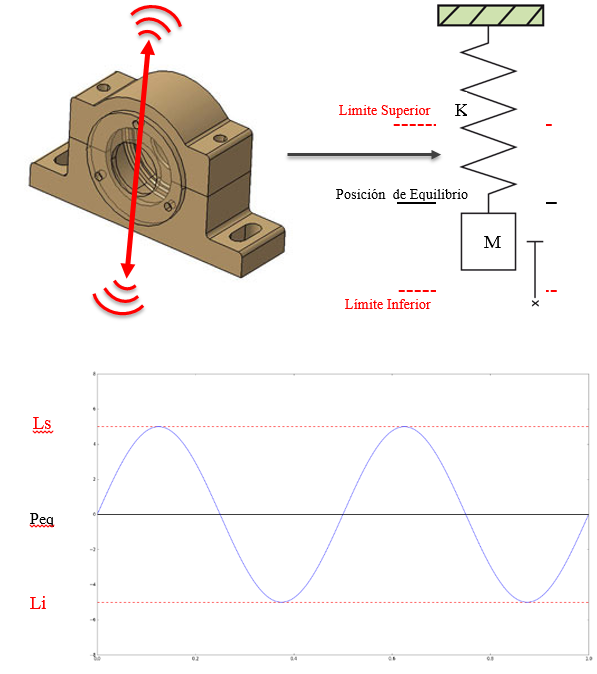
\includegraphics[width=0.7\textwidth]{ejemplovibracioncajarod}
			\caption{Desplazamiento vibratorio vertical de la caja del rodamiento}
			\label{fig:ejvibracionrod}
		\end{figure}
			
		El movimiento del punto superior de la caja se puede representar mediante tres magnitudes, posición, velocidad y aceleración; y al ser armónica esta señal puede caracterizarse mediante dos paramentos, \textbf{amplitud} y \textbf{frecuencia}. \\
			
		En la Imagen \ref{fig:ejvibracionrod} se ejemplifica lo anterior, la caja de rodamientos de una maquina la cual está vibrando verticalmente. Si la superficie de la caja del cojinete se mueve (o vibra) significa que su unión a la base es elástica, por lo que el sistema se puede modelar mediante un sistema masa-resorte. Para la forma de onda de la imagen se puede apreciar una amplitud de valor pico de 5 y una frecuencia de 2 [Hz] (dos oscilaciones en el intervalo de un segundo). La amplitud suele expresarse de tres maneras diferentes dependiendo del fenómeno que se esté estudiando.
		\begin{enumerate}
			\item  \underline{Valor pico}: Es el mayor valor que alcanza la vibración, ya sea hacia el positivo o el negativo, en el caso de las vibraciones armónicas, este valor es igual tanto al positivo como al negativo.
			\item \underline{Valor pico a pico}: : es la diferencia entre el mayor valor alcanzado en el eje positivo y el mayor valor alcanzado en negativo.
			\item \underline{Valor RMS}: Se define como la raíz del valor promedio de los valores instantáneos de la vibración elevados al cuadrado.
			\begin{equation}
			\sqrt{\frac{1}{n}(x_1^{2}+x_2^{2}+x_3^{2}+\cdot\cdot\cdot+x_n^{2})}
			\end{equation}
		\end{enumerate}
		\subsection{Medición de la Vibración} 
			Las etapas a seguir para la medición y análisis de las vibraciones se clasifican en las siguientes partes:
			\begin{enumerate}
				\item \textbf{\textit{Transductora}}: Etapa donde el sensor de vibraciones transforma la señal análoga (vibración del equipo) en una señal eléctrica \textbf{proporcional} a la magnitud medida.
					
				\item \textbf{\textit{Acondicionamiento de la señal eléctrica}}: Algunas señales entregadas por el sensor no pueden ser registradas o introducidas directamente, es decir, necesitan ser acondicionadas previamente. Por ejemplo, la señal de un sensor de vibración necesita de una amplificación de la señal en orden de ser percibida. Por lo general los sensores de aceleración (acelerómetros piezoeléctricos) usados en la industria vienen con un preamplificador (ICP, integrated circuit piezoelectric) de la señal integrado, haciendo que esta etapa no sea percibida.
					
				\item \textbf{\textit{Procesamiento  y medición}}: Etapa fundamental del análisis de vibración, pues esta etapa consiste en usar técnicas o procedimientos para sacar la mayor información de la información, el procesamiento clásico de la medición de vibraciones es el análisis de frecuencia mediante el uso de la transformada de Fourier. Otro ejemplo de procesamiento y medición es capturar los valores RMS, valor pico, valor pico-pico.
					
				\item \textbf{\textit{Registro}}: Consiste en guardar (registrar) los datos medidos y procesados, este puede ser directamente en el equipo transductor como en un Computador.
			\end{enumerate} 
			Existen diferentes tipos de sensores de vibraciones típicos, dentro de los cuales los de uso más común son
			\begin{enumerate}
				\item Desplazamiento relativo sin contacto
				\item Desplazamiento relativo sin contacto
				\item Sensor de velocidad o velocímetro
				\item Sensor de aceleración o acelerómetro.
			\end{enumerate}
			Para efectos de medición, se utilizará un sensor de aceleración (\ref{fig:acellpartes}) piezoeléctrico, el cual es el tipo de sensor usado en mayoría. El principio de funcionamiento son los materiales piezoeléctricos (como el cuarzo) que tienen la propiedad de que al aplicarles una fuerza externa en dirección de su polarización se genera una carga eléctrica entre sus superficies, la cual es proporcional a la fuerza aplicada y por ende, a su aceleración. \\			
			\begin{figure}[t]
				\centering
				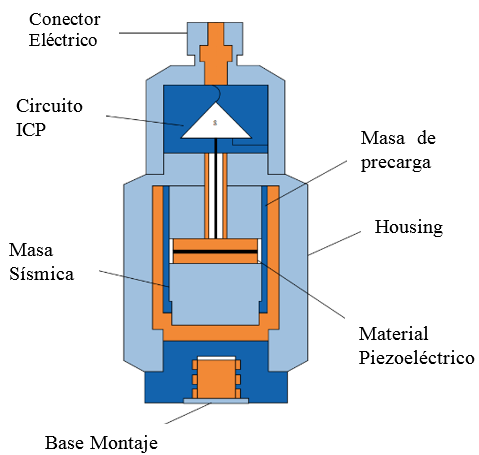
\includegraphics[width=0.7\textwidth]{partesacelerometro}
				\caption{Esquema de un acelerometro y sus partes principales}
				\label{fig:acellpartes}
			\end{figure}
		
		\subsection{Transformada de Fourier}
			Uno de los conceptos fundamentales en la etapa de procesamiento de la señal captada, es la transformada de Fourier, la cual se usa en el estudio de funciones (o señales) y como estas pueden descomponerse en funciones trigonométricas o exponenciales con frecuencias específicas. La transformada de Fourier se realiza mediante el uso del algoritmo llamado FFT (Fast Fourier Transform), que permite computar de manera más rápida la transformada discreta de Fourier (\ref{fig:medicionfft}) \cite{fourieranalysis}.\\
			\begin{figure}[t]
				\centering
				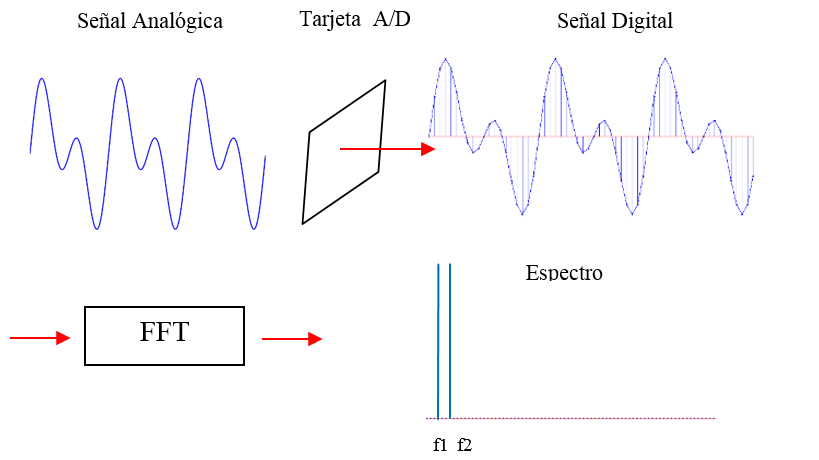
\includegraphics[width=\textwidth]{medicionfft}
				\caption{Calculo de una FFT desde la medición}
				\label{fig:medicionfft}
			\end{figure}
		
		Para entender esta transformación, se procederá a explicar dos conceptos fundamentales
		\begin{enumerate}
			\item \textbf{Serie de Fourier}: Si una función es periódica, puede ser descrita como una \textit{suma discreta} de funciones trigonométricas o exponenciales con frecuencias específicas
			
			\item \textbf{Transformada de Fourier}: Generalización de la serie de Fourier, donde la función a describir no tiene que ser específicamente periódica, y se describe como una \textit{integral continua} de funciones trigonométricas o exponenciales con la posibilidad de tener frecuencias continuas.
		\end{enumerate}
	
		\subsubsection{Serie de Fourier}
			Consideremos una función $f(x)$ periódica en un intervalo $0 \leq x\leq L$ como la de la figura \ref{fig:funcperiodica}
			\begin{figure}[H]
				\centering
				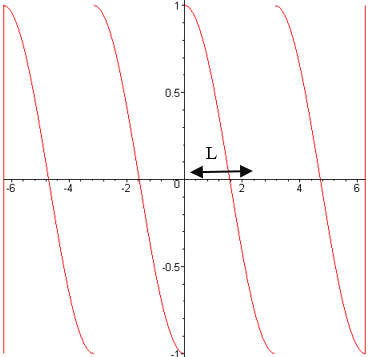
\includegraphics[width=0.5\textwidth]{funcionperiodica}
				\caption{Ejemplo función periódica}
				\label{fig:funcperiodica}
			\end{figure}	
			\newpage
		
			Asumiendo periodicidad $0\leq x \leq L$ , la serie de Fourier se expresa como:
			
			\begin{equation}			
			f\left(x\right)=a_0+\sum_{n=1}^{\infty{}}\left[a_n\cos{\left(\frac{2\pi{}nx}{L}\right)}+b_n\sin{\left(\frac{2\pi{}nx}{L}\right)}\right]
			\label{eq:seriedefourier}
			\end{equation}
			
			Se debe notar que la sumatoria parte desde n=1 puesto que para $n=0$ la parte de la sumatoria que tiene la función seno se hace cero y el coseno al ser $0$ es $1$, teniendo solo un parámetro constante ($a_0$). Otro aspecto que se puede observar directamente de la fórmula es que para el termino $n=1$ se tiene un periodo de L, incrementando el valor de $n$ el periodo de cada termino sucesivo es de $\frac{L}{2}$, $\frac{L}{3}$, $\frac{L}{4}$ …, es decir, la transformada respeta el periodo de la señal original, teniendo como máximo un periodo de 1 para el caso de $n=1$.
			
			Para el cálculo de los términos $a_0$ 〖$a_n$,$b_n$ se basan en la ortogonalidad en funciones, específicamente para las funciones trigonométricas se tienen las siguientes identidades:
			
			\begin{equation}			
				\centering				
				\int_0^L\sin{\left(\frac{2\pi{}nx}{L}\right)\cos{\left(\frac{2\pi{}mx}{L}\right)}}dx=0				
				\label{eq:proptrig1}
			\end{equation}		
				
			\begin{equation}
				\centering
				\int_0^L\cos{\left(\frac{2\pi{}nx}{L}\right)\cos{\left(\frac{2\pi{}mx}{L}\right)}}dx=\frac{L}{2}\delta_{nm}
				\label{eq:proptrig2}
			\end{equation}
			
			\begin{equation}
				\centering
				\int_0^L\sin{\left(\frac{2\pi{}nx}{L}\right)\sin{\left(\frac{2\pi{}mx}{L}\right)}}dx=\frac{L}{2}\delta_{nm}
				\label{eq:proptrig3}
			\end{equation}
			
			Donde $\delta_{nm}$ es un delta de Kronecker, el cual se define como 1 si $n=m$ y 0 en cualquier otro caso. Con esta propiedad, para obtener los factores, se calculan las siguientes integrales:
			
			\begin{equation}
				\centering
				\int_0^Lf\left(x\right)\ dx=a_0L\ \rightarrow{}a_0=\frac{1}{L}\ \int_0^Lf(x)
				\label{eq:obta0}
			\end{equation}
			
			\begin{equation}
				\centering
				\int_0^Lf\left(x\right)\cos{\left(\frac{2\pi{}mx}{L}\right)}=\frac{L}{2}a_0\rightarrow{}a_m=\frac{2}{L}\int_0^Lf\left(x\right)\cos{\left(\frac{2\pi{}mx}{L}\right)\ dx}
				\label{eq:obtam}
			\end{equation}
			
			\begin{equation}
				\int_0^Lf\left(x\right)\sin{\left(\frac{2\pi{}mx}{L}\right)}=\frac{L}{2}a_m\rightarrow{}b_m=\frac{2}{L}\int_0^Lf\left(x\right)\sin{\left(\frac{2\pi{}mx}{L}\right)\ dx}
				\label{eq:obtbm}
			\end{equation}
			
			Esta manera de expresar la serie de Fourier corresponde a la Serie trigonométrica de Fourier la cual puede ser escrita de manera compleja con la fórmula de Euler, obteniendo la Serie exponencial de Fourier $e^{ix} $= $cos(x) + i sin(x)$ obteniendo:
			\begin{equation}
				{f\left(x\right)=\ \sum_{n=-\infty{}}^{\infty{}}C_ne^{\frac{i\ 2\pi{}\ nx}{L}}}				
			\end{equation}
			\begin{equation}
				C_n=\frac{1}{L}\int_{-\infty{}}^{\infty{}}f(x)e^{\frac{-i\ 2\pi{}\
						nx}{L}}dx
				\label{eq:expfourier}
			\end{equation}
			
			Se puede observar de la ecuación \ref{eq:expfourier} que la sumatoria va desde $-\infty$  a $\infty$, a diferencia del caso trigonométrico donde los valores negativos de $n$ dan valores redundantes.
			
		\subsubsection{Transformada de Fourier}
		
			El cálculo de la Serie de Fourier se fundamenta solo en funciones periódicas de periodo L. Si la serie no es periódica la Transformada de Fourier de manera directa falla, sin embargo, si se considera el periodo de la función $\frac{-L}{2} \leq x \leq \frac{L}{2}$ con $ L \rightarrow \infty $  la función pasa a no tener periodo, o más bien un periodo que tiende al infinito, pasando de una serie discreta a una transformada continua, tomando como punto de partida la serie exponencial de Fourier
			
			\begin{equation}
				f\left(x\right)=\ \sum_{n=-\infty{}}^{\infty{}}C_ne^{\frac{i\ 2\pi{}\ nx}{L}}\ \
				\ \ \ \ \ \ donde\ \ \ \ \ \ \ \
					C_n=\frac{1}{L}\int_{-\frac{L}{2}}^{\frac{L}{2}}f(x)e^{\frac{-i\ 2\pi{}\ nx}{L}}
			\end{equation}
			
          	Si se define $$k_n= \frac{2\pi n}{L}$$ y su diferencia $$dk_n = \frac{2\pi dn}{L}$$ se obtiene
			\begin{equation}
				f\left(x\right)=\ \sum_{n=-\infty{}}^{\infty{}}C_ne^{ik_nx}\left(\frac{L}{2\pi{}}{dk}_n\right)
			\end{equation}
			
			Como el diferencial es muy pequeño, la sumatoria se convierte en una integral
			\begin{equation}
				f\left(x\right)=\ \int_{-\infty{}}^{\infty{}}C(k_n)e^{ik_nx}\left({dk}_n\right)
			\end{equation}
			
			Para obtener $C(k_n )$  se tiene la siguiente igualdad
			
			\begin{equation}
				\left. C(k_n\right.)=\frac{L}{2\pi{}}C_n=\frac{1}{2\pi{}}\int_{-\infty{}}^{\infty{}}f(x)e^{-ik_nx}dx
			\end{equation}
			
			Finalmente se obtienen las siguientes dos relaciones:
			\begin{equation}
				f\left(x\right)=\int_{-\infty{}}^{\infty{}}C\left(k\right)e^{ikx}{dk}_n\ \
			\end{equation}
		    
		    \begin{equation}
		    f\left(x\right)=\int_{-\infty{}}^{\infty{}}C\left(k\right)e^{ikx}{dk}_n\ \
		    \label{eq:transformadafourier}
		    \end{equation}
			Donde de la ecuación \ref{eq:transformadafourier} se le conoce como transformada de Fourier la cual nos dice que $f(x)$ indica cuanto de la función $C(k)$ está hecha de $e^{-ikx}$. 
		\subsubsection{Transformada discreta de Fourier}
			La transformada de Fourier tiene un trasfondo puramente matemático, y es aplicable solo a funciones continuas, Es por esto que se introduce el concepto de Transformada Discreta de Fourier, computada mediante el algoritmo FFT (ingles \textit{Fast Fourier Transform}).
			
			\begin{equation}
				X\left[k\right]=\ \sum_{n=0}^{N-1}x[n]e^{-\frac{2\pi{}i}{N}kn}
				\label{eq:discretafourier}
			\end{equation}
			
			Uno de los grandes limitantes es la gran cantidad de operaciones que deben hacerse para su cálculo, específicamente $ O( n^2 ) $. Mediante manipulación matemática, en el año 1965, James Cooley y John Tukey publicaron una manera general de un algoritmo capaz de reducir el número de operaciones a $O(n log(n)$ (figura \ref{fig:diffftdft}), existen numerosos algoritmos computacionales para el cálculo de la FFT, uno de los más famosos y gratuitos es el FTTW (Fastest Fourier Transform of the West).
			\begin{figure}
				\centering
				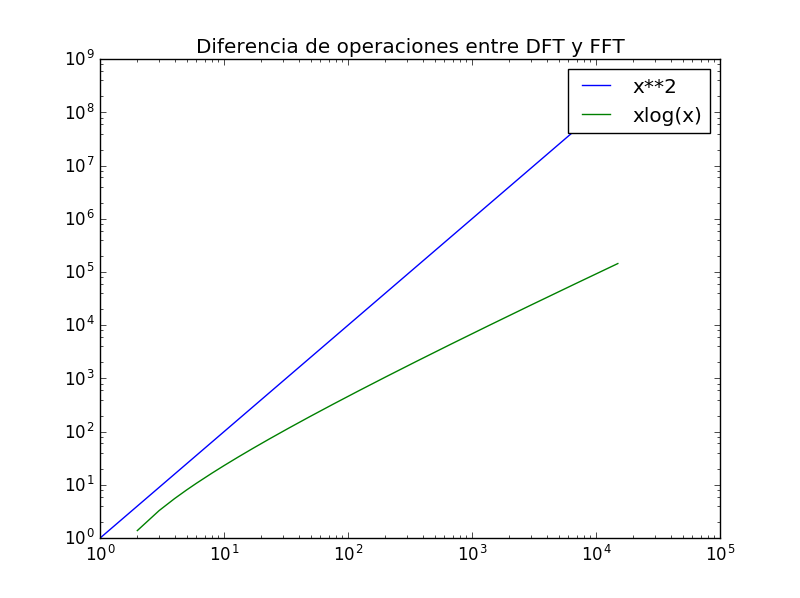
\includegraphics[width=0.5\textwidth]{DiferenciaentreDFTyFFT}
				\caption{Diferencia en operaciones entre FFT y DFT}
				\label{fig:diffftdft}
			\end{figure}
		\subsection{Consideraciones al adquirir datos para computar FFT}
			\subsubsection{\textbf{Aliasing}}
				El aliasing es un problema que ocurre al medir frecuencias superiores a la frecuencia de sampling, específicamente y según el teorema de Nyquist la frecuencia de sampleo debe ser al menos el doble de la frecuencia máxima encontrada en la señal medida, es decir:
				\begin{equation}
					f_{sampleo} \leq 2\dot f_{maximo}
				\end{equation}
				Este problema (aliasing) provoca que la FFT tome un valor de frecuencia diferente (menor) al real, como se muestra en la figura \ref{fig:aliasing}
				\begin{figure}
					\centering
					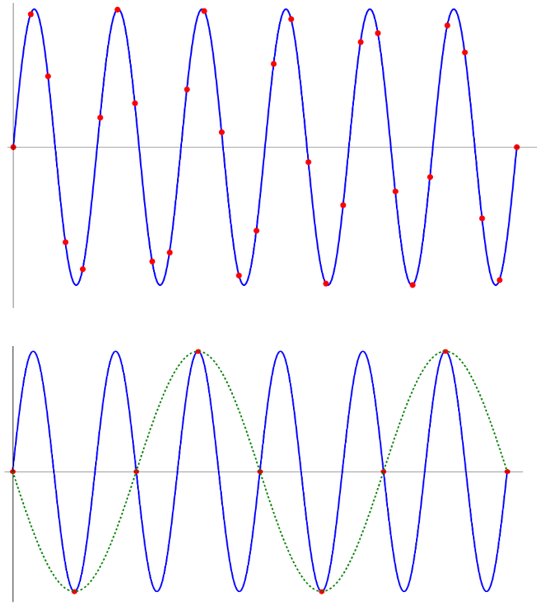
\includegraphics[width=0.5\linewidth]{badnyquist}
					\caption{Problema Aliasing (Linea verde)}
					\label{fig:aliasing}
				\end{figure}
			
				En la primera imagen se aprecia (\ref{fig:aliasing}) (puntos rojos) que el sampling es mayor a la frecuencia de la Onda, al usar FFT, la frecuencia corresponderá a la frecuencia real de la onda, empero el segundo caso, en el cual solo se alcanza a tomar una muestra por periodo, al calcular la FFT, la frecuencia sería la de una onda menor (en este caso de 2[Hz]). Para mitigar este efecto, los transductores deben incluir un filtro pasa bajo previa conversión análoga/digital de la señal para así eliminar toda vibración sobre la frecuencia de corte seleccionada, a este filtro se le llama filtro antialiasing.
			\subsubsection{Fugas Laterales}
				La transformada de Fourier supone que el rango de tiempo es de registro infinito, en la práctica este criterio se vuelve prácticamente imposible de ejecutar, ya que un recolector de datos solo puede tomar un intervalo finito de tiempo, esto genera que la transformada de Fourier para una onda sinusoidal no sea una sola línea en el espectro sino que pasa a ser un gráfico con forma de lóbulos \ref{fig:fugaslat}, centrada en la frecuencia de la onda. \\
				\newpage
				\begin{figure}
					\centering
					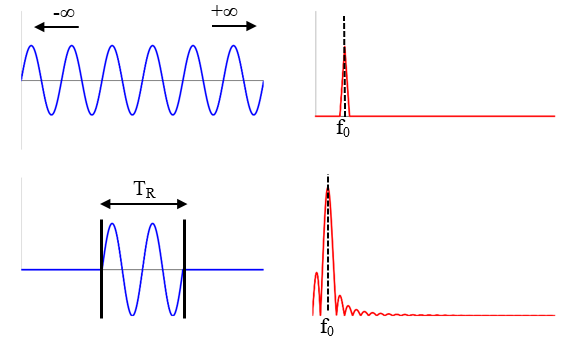
\includegraphics[width=0.9\linewidth]{fugaslat}
					\caption{Efecto de fugas laterales}
					\label{fig:fugaslat}
				\end{figure}
				Otro efecto presente en la adquisición de datos ocurre cuando los datos no alcanzan a tomar un periodo entero de datos, pues la FFT replica la señal obtenida (ya que esta se basa en una serie infinita), si no se toma un periodo completo de la señal, esta al replicarla queda con saltos bruscos, como se muestra en la figura \ref{fig:periodoinc}				
				
				
				\begin{figure}[H]
					\centering
					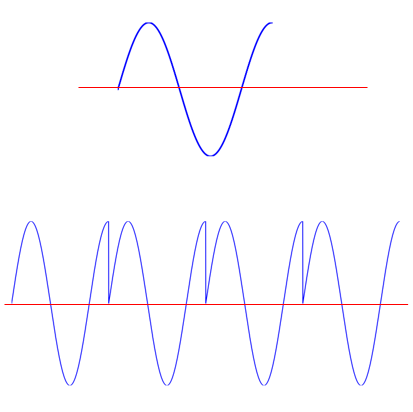
\includegraphics[width=0.5\linewidth]{periodoinc}
					\caption{Onda replicada de periodo incompleto (se producen cambios bruscos en la forma de onda)}
					\label{fig:periodoinc}
				\end{figure}
				\newpage
				Este efecto hace que en el espectro ya no aparezca una componente a la frecuencia correspondiente, sino que aparecen fugas laterales. La imágen \ref{fig:windowing1} y \ref{fig:windowing2} muestra un ejemplo de este problema. La primera señal corresponde a una onda de $10 [Hz]$ captada por 10 segundos, la segunda a una señal de $10.25 [Hz]$.
				\begin{figure}
					\centering
					\begin{subfigure}[b]{\linewidth}
						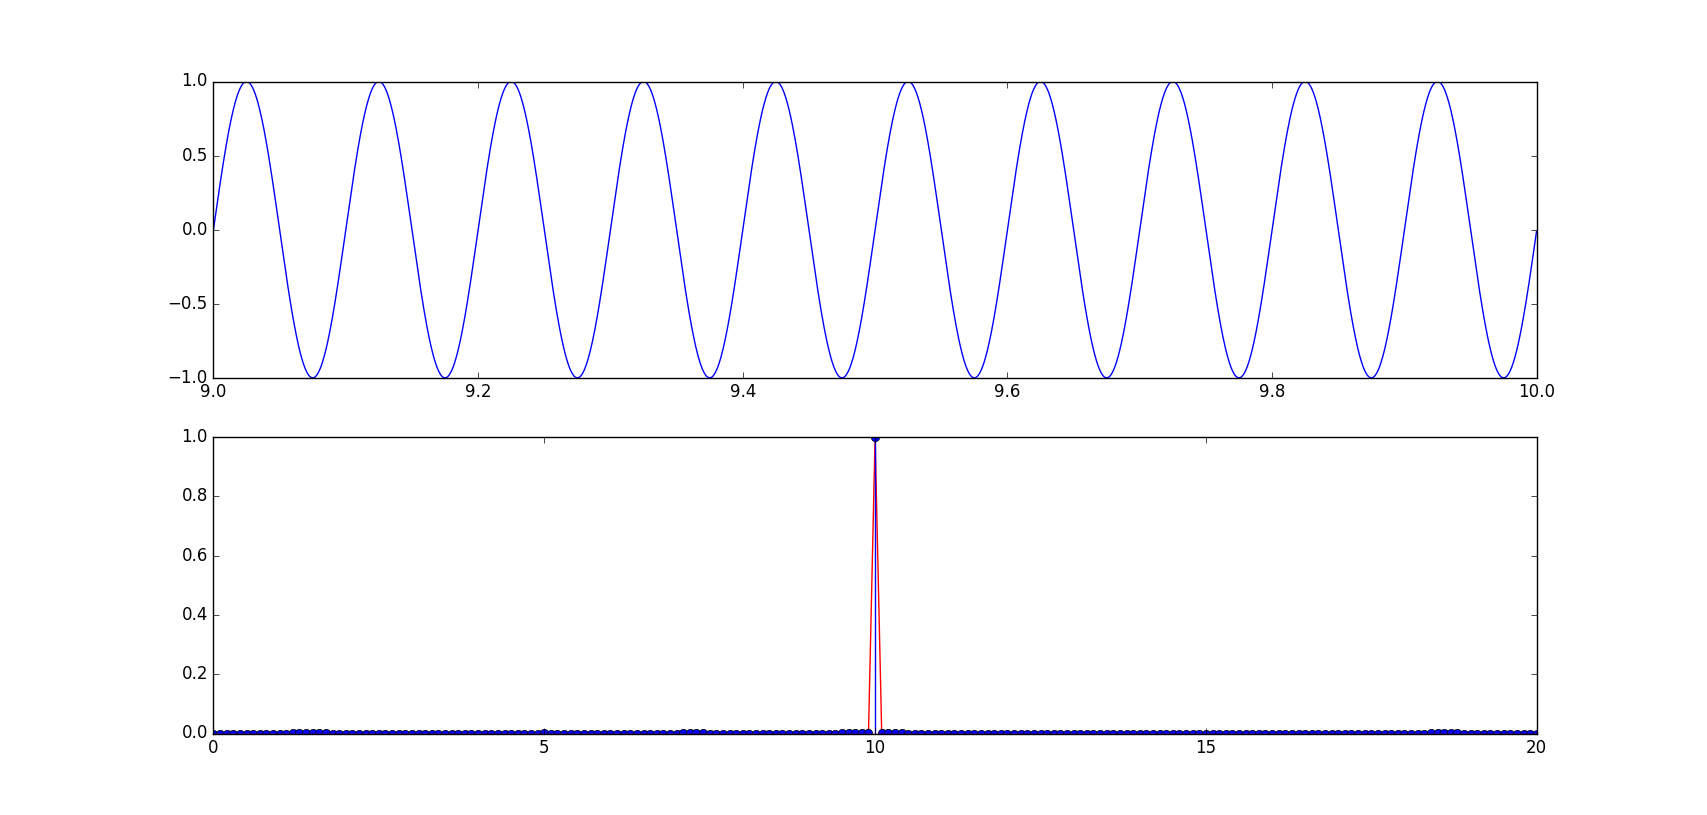
\includegraphics[width=0.9\linewidth]{windowproblem1}
						\caption{Adquisicion de una onda de periodo completo}
						\label{fig:windowing1}
					\end{subfigure}
					\begin{subfigure}[b]{\linewidth}
						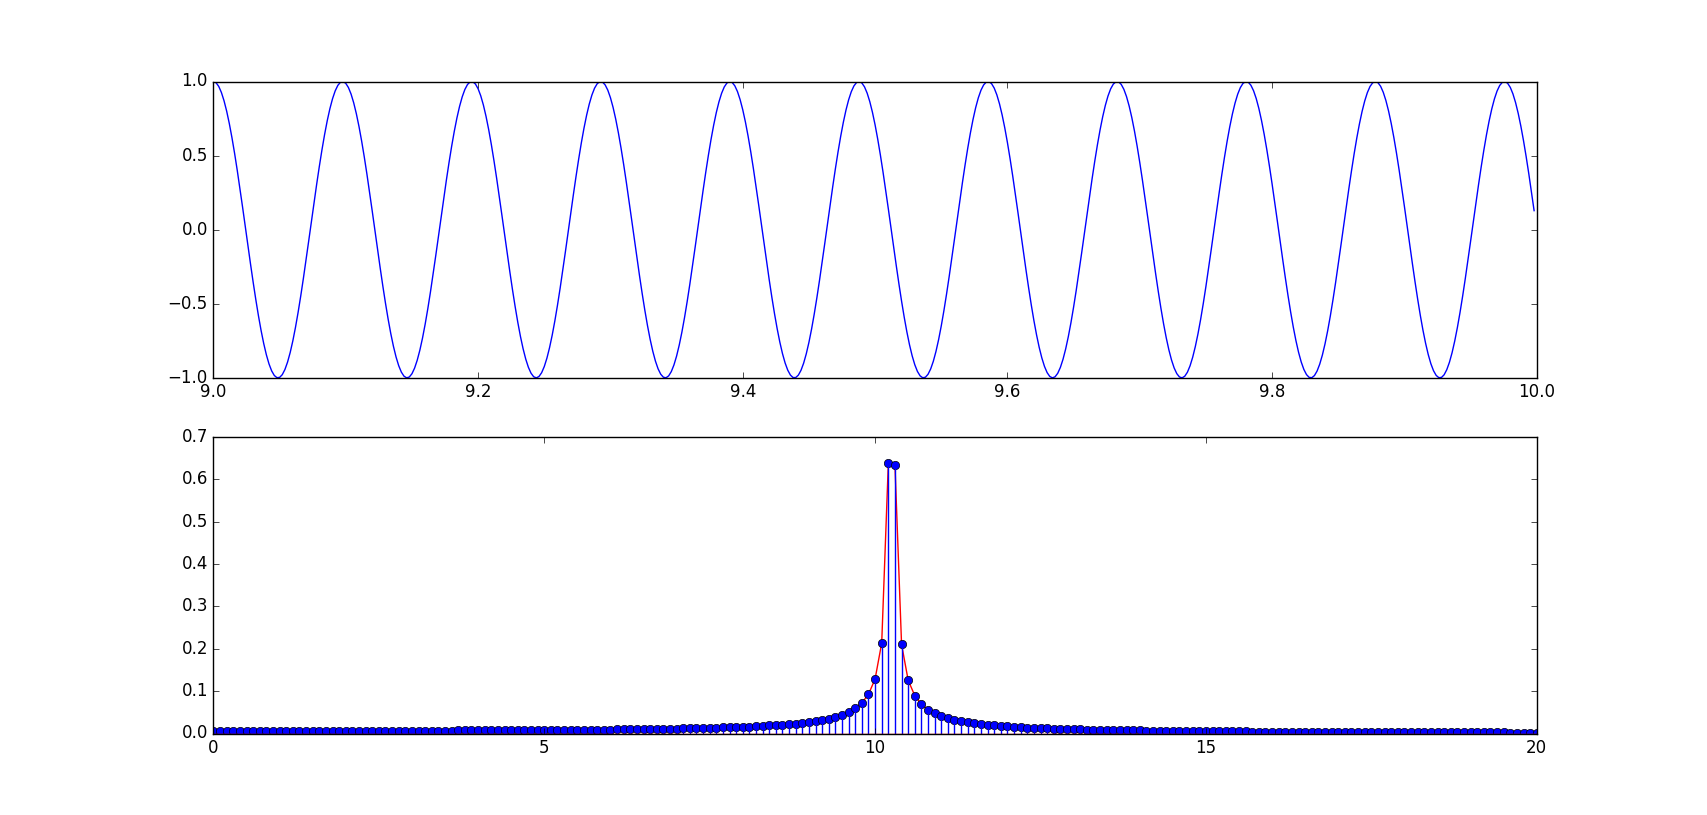
\includegraphics[width=0.9\linewidth]{windowproblem22}
						\caption{Adquisicion de una onda de periodo incompleto}
						\label{fig:windowing2}
					\end{subfigure}
					\caption{Fugas laterales en registro no periódico}
					\label{fig:comparacionfuglat}						
				\end{figure}
				\newpage
				\begin{figure}
					\centering
					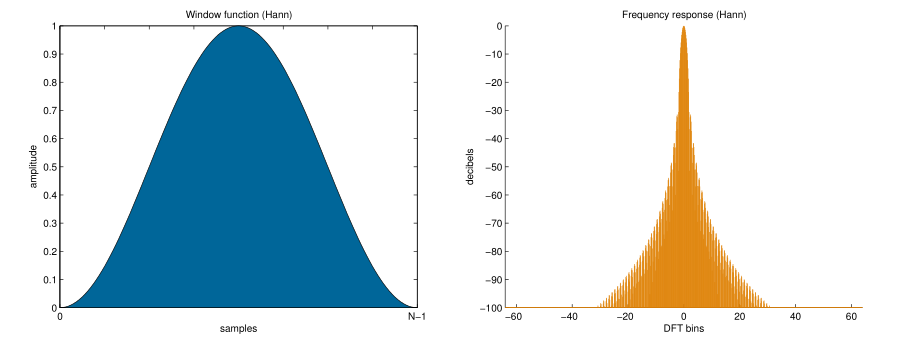
\includegraphics[width=0.9\linewidth]{hann}
					\caption{Gráfico de ventana Hann (fuente: Wikipedia)}
					\label{fig:hannwindow}					
				\end{figure}
				Para mitigar este efecto de las fugas laterales es mediante la introducción de las funciones ventanas, que hacer que la función en ambos extremos converge a 0 haciendo que al juntar el final de la señal periódica con el inicio de ella misma, se haga de manera suave (es decir, no existan cambios o saltos en la función). Existen diferentes tipos de ventanas, siendo el mas usado en el análisis de vibración la ventana Hann (eq: \ref{eq:hann},fig: \ref{fig:hannwindow}), una vez definida la ventana, basta con hacer el producto entre la señal y la ventana para obtener la nueva función a la cual se le aplicara la transformada discreta de Fourier. Una limitante de este proceso es que agrega un grado de distorsión a la forma de onda que se esté analizando, bajo la forma de una modulación en amplitud (aparecerán de misma manera bandas laterales). Otro inconveniente que posee este tipo de ventana es que la amplitud de la señal pesada por el ponderado de la ventana Hann es menor que la señal original \cite{white2010introduction}, en esencia se quita la mitad de la señal por el proceso (pues la señal se lleva a cero), esta perdida de amplitud se corrige multiplicando los niveles del espectro por dos en todo el intervalo de muestreo. Otro factor importante es que este tipo de ponderación debe hacerse en señales continuas y nunca con transientes ya que esta ventana distorsiona la forma de onda.
				\begin{equation}										
					v(n) = a_{0} - a_{1} \cos (\frac{2\pi n}{N-1}) \\				
					a_{0}=0.50 ; a_{1}=0.50			
					\label{eq:hann}
				\end{equation}
			    
				Tomando en cuenta la forma de onda de la figura \ref{fig:windowing2} se multiplica la señal por la ventana Hann obteniendo así una nueva gráfica (figura \ref{fig:windowing3}) estrechez en las fugas laterales, también es posible ver la disminución en la amplitud de la señal, pues esta no a sido manipulada para mostrar los efectos de esta.
				\begin{figure}[H]
					\centering
					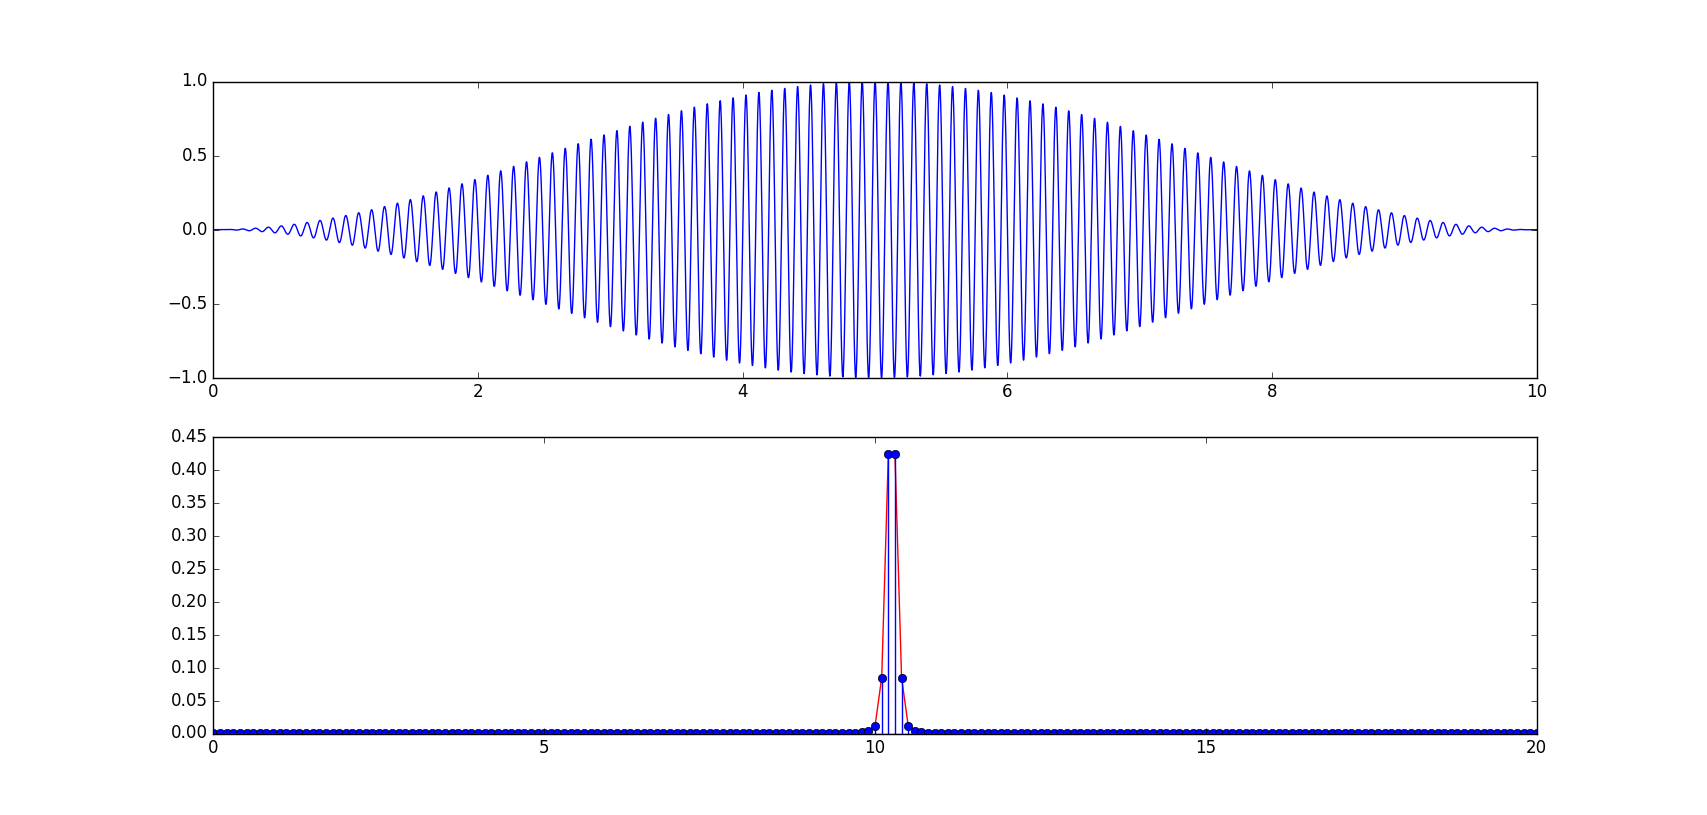
\includegraphics[width=0.9\linewidth]{windowproblemhann}
					\caption{Efecto de la ponderación de la señal por la ventana Hann}
					\label{fig:windowing3}	
				\end{figure}
		 		Existen varias ventanas de ponderación aplicables a señales, dependiendo de lo que se esté analizando se utiliza de mejor manera el tipo de ventana, algunas de estas funciones se llaman: Hann, Hamming, Blackman,Blackman-Harris, Barlett, Flat top, Gauss, Kaiser (\href{https://es.wikipedia.org/wiki/Ventana_(funcion)}{link: Wikipedia}).
		 	\subsection{Densidad Espectral}
		 		La densidad espectral de una señal nos da cuenta de como esta distribuida la potencia o la energía de dicha señal en cada frecuencia de la cual está formada. Para procesos transcientes en el tiempo (aquellos que empiezan y terminan en cero en amplitud) es posible usar densidad espectral con relación a su energía (ejemplo, prueba de impacto). En el caso de señales continuas y estacionarias donde la cantidad de energía medida es proporcional al tiempo de observación, deben ser medidas en unidades de potencia, es decir, de energía por unidad de tiempo.\\
		 		Básicamente la PSD (\textbf{Power} Spectrum Density) se calcula como el valor esperado de la transformada de Fourier con la señal al cuadrado (potencia) (ecuación \ref{eq:psd})
		 		\begin{equation}
			 		S_{xx}(\omega) = \lim_{T\to\infty}(\textbf{E}\lvert \hat{x}_T(\omega)\rvert^2)
			 		\label{eq:psd}
		 		\end{equation}
		 		donde $S_{xx}(\omega)$ es el valor de la PSD.
		 		Uno de los métodos para aproximar la PSD es el algoritmo propuesto por P.D Welch \cite{Welch1967}, el cual propone calcular la PSD a través de la Transformada de fourier en segmentos de la señal original (periodogramas) para luego promediar cada uno de ellos. Cada segmento de la señal original es multiplicada por una función ventana. Los parámetros para el calculo de la PSD mediante el método de Welch son:
		 		\begin{itemize}
		 			\item \textbf{x}: Arreglo con los datos de la serie de tiempo
		 			\item \boldmath{$f_s$}: frecuencia de sampleo de la serie de tiempo
		 			\item \textbf{window}: Ventana a aplicar sobre x
		 			\item \textbf{nperseg}: Número de puntos de la serie de tiempo por segmento
		 			\item \textbf{noverlap}: Número de puntos a superponer entre segmentos
	 			\end{itemize}
		 		Los cuales devuelven dos series de datos:
		 		\begin{itemize}
		 			\item \textbf{f}: arreglo con las frecuencias de sampleo.
		 			\item \boldmath{$P_{xx}$}: PSD del arreglo x.		
		 		\end{itemize}
	 		\subsection{Modelos clásicos de fallas en equipos vibratorios}
	 			La siguiente sección tiene por objetivo mostrar los principales modos de falla de equipos rotatorios conocidos, estos equipos deben tener la condición de girar sobre las 200 revoluciones por minuto (RPM) debido a que con esas revoluciones las fuerzas dinámicas son capaces de generar patrones que pueden ser comparables para distintos tipos de máquinas.
	 			\subsubsection{Síntomas vibratorios del desbalanceo}
	 				El desbalanceo de masas es la causa más común de vibraciones. El desbalanceo es principalmente un desfase o corrimiento del centro de masas del rotor con su eje de rotación o geométrico. Algunas causas de desbalanceo son:
	 				\begin{itemize}
	 					\item Desgaste no simétrico del material
	 					\item Dilataciones no simétricas
	 					\item Deformaciones no simétricas cuando fija a su velocidad de operación
	 					\item Adherencia de material en el rotor durante su operación 
	 					\item Pernos de diferente masa dentro del rotor
	 					\item Problemas en el diseño del chavetero
	 				\end{itemize}
	 				Estas causas generan dos posibles cambios en el rotor
	 				\begin{enumerate}
	 					\item \textbf{Punto Pesado}: El cual corresponde al punto en el cual la masa desbalanceada se localiza
	 					\item \textbf{Cantidad de desbalanceo (U)}: Es la medida cuantitativa de desbalanceo en un rotor, definido por: $$ U= m \cdot r $$
	 					donde $m$ es la masa desbalanceada y $r$ es la distancia de la masa desbalanceada al eje de rotación.
	 				\end{enumerate} 
	 				Cuando el valor de U aumenta hace que la manifestación del desbalanceo sea mayor, aumentando considerablemente la magnitud de la componente 1X junto con componentes a la 2X y 3X (Estas en menor amplitud,bajo el $10\% $ de la 1X) (figura: \ref{fig:desbgrafico}) en el espectro de frecuencia (donde 1X corresponde a la frecuencia) por lo que en el espectro vibratorio, este síntoma se manifiesta con una componente predominante a 1X, este problema puede observarse de manera fácil comprobando la evolución de la componente 1X a través del tiempo, a medida que esta crece en amplitud, suele relacionarse con un aumento en el desbalanceo. Debe tenerse presente además que a revoluciones altas de giro del rotor (sobre 200[Hz]) siempre aparecerá la componente 1X del sistema, pues este se debe al desbalanceo residual el cual es imposible omitir en su totalidad.
	 				\begin{figure}
	 					\centering
	 					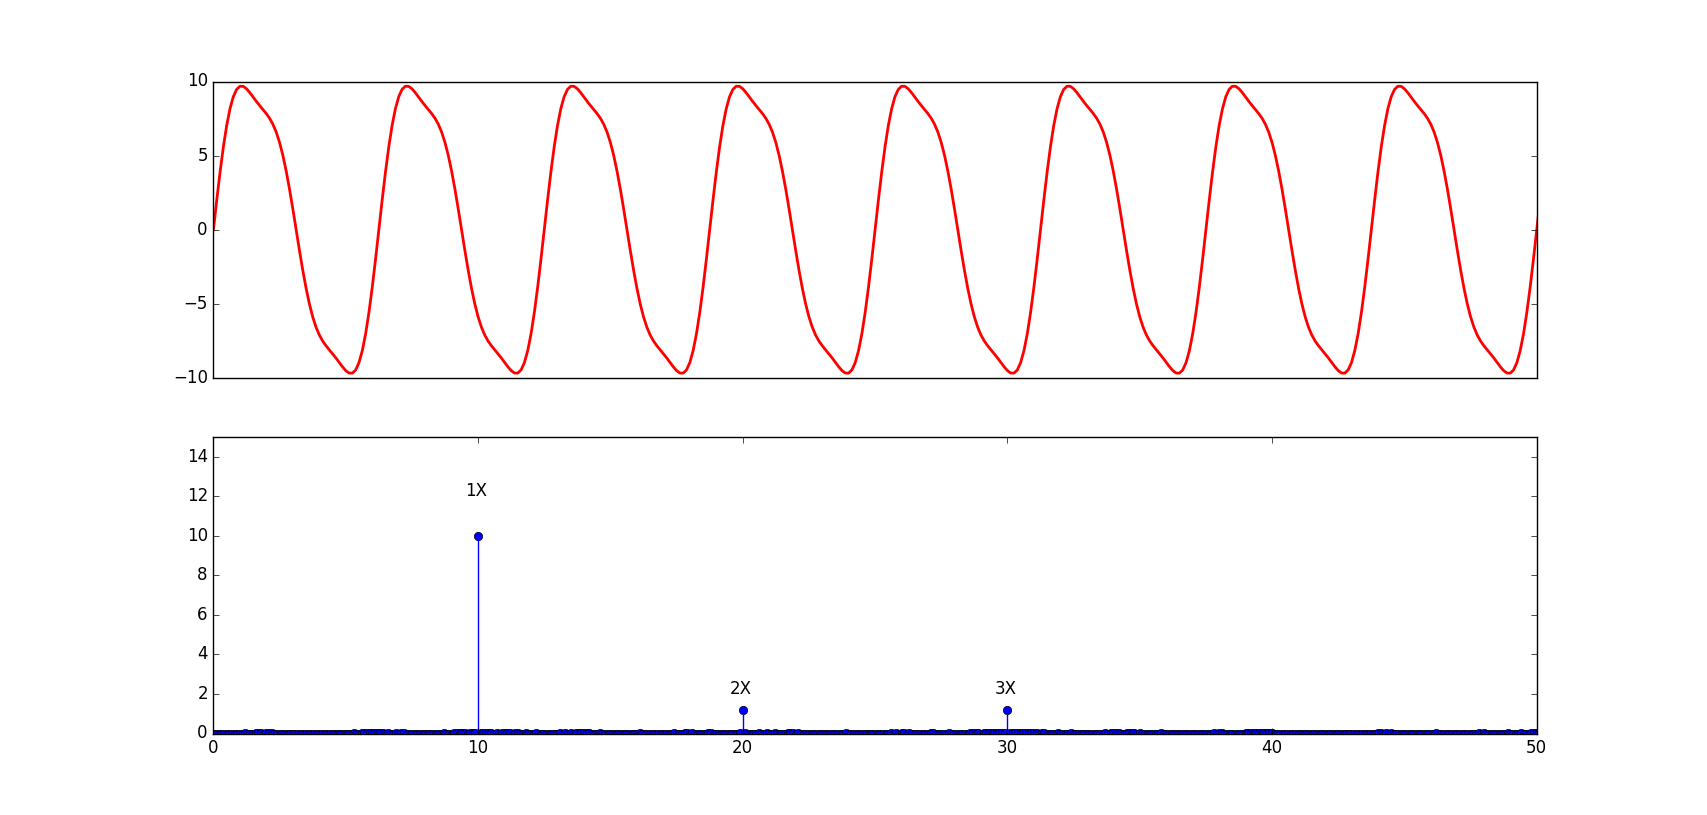
\includegraphics[width=0.9\linewidth]{desbalanceoplot}
	 					\caption{Forma de Onda y FFT característicos de desbalanceo}
	 					\label{fig:desbgrafico}
	 				\end{figure}
 				\subsubsection{Síntomas vibratorios del desalineamiento}
 					El desalineamiento de acoples es una condición de falla donde los componentes de una máquina (conectados) no están conectados de manera co-lineal en su punto de unión en su periodo de funcionamiento. Existen diferentes tipos de desalineamiento en máquinas
 					\begin{itemize}
 						\item Desalineamiento paralelo (figura: \ref{fig:desparalelo})
 						\item Desalineamiento angular (figura: \ref{fig:desangular})
 						\item Desalineamiento mixto (figura: \ref{fig:desmixto})
 					\end{itemize}
	 				\begin{figure}
	 					\centering
	 					\begin{subfigure}[b]{0.4\textwidth}
	 						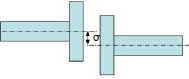
\includegraphics[width=\textwidth]{desalineamientparalelo}
	 						\caption{Desalineamiento paralelo}
	 						\label{fig:desparalelo}
	 					\end{subfigure}			    
	 					\begin{subfigure}[b]{0.4\textwidth}
	 						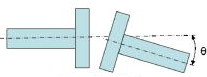
\includegraphics[width=\textwidth]{desalineamientoangular}
	 						\caption{Desalineamiento angular}
	 						\label{fig:desangular}
	 					\end{subfigure}
	 					\begin{subfigure}[b]{0.5\textwidth}
	 						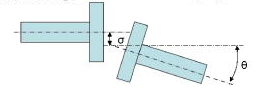
\includegraphics[width=\textwidth]{desalineamientocombinado}
	 						\caption{Desalineamiento combinado}
	 						\label{fig:desmixto}
	 					\end{subfigure}
	 				
	 					\caption{Tipos de desalineamientos}
	 					\label{fig:tiposdedes}
	 				\end{figure}
	 				Este tipo de problema tiene su origen principalmente al momento del montaje, también suele presentarse una evolución del desalineamiento durante su operación debido principalmente a deformaciones debido a los esfuerzos por carga de la máquina.
	 			
	 				En el espectro vibratorio, este tipo de falla suele presentarse con componentes predominantes en la 1X 2X 3X, dependiendo del grado de severidad del desalineamiento pueden aparecer aún mas armónicos (4X a 11X)
	 				\begin{figure}
		 				\centering
		 				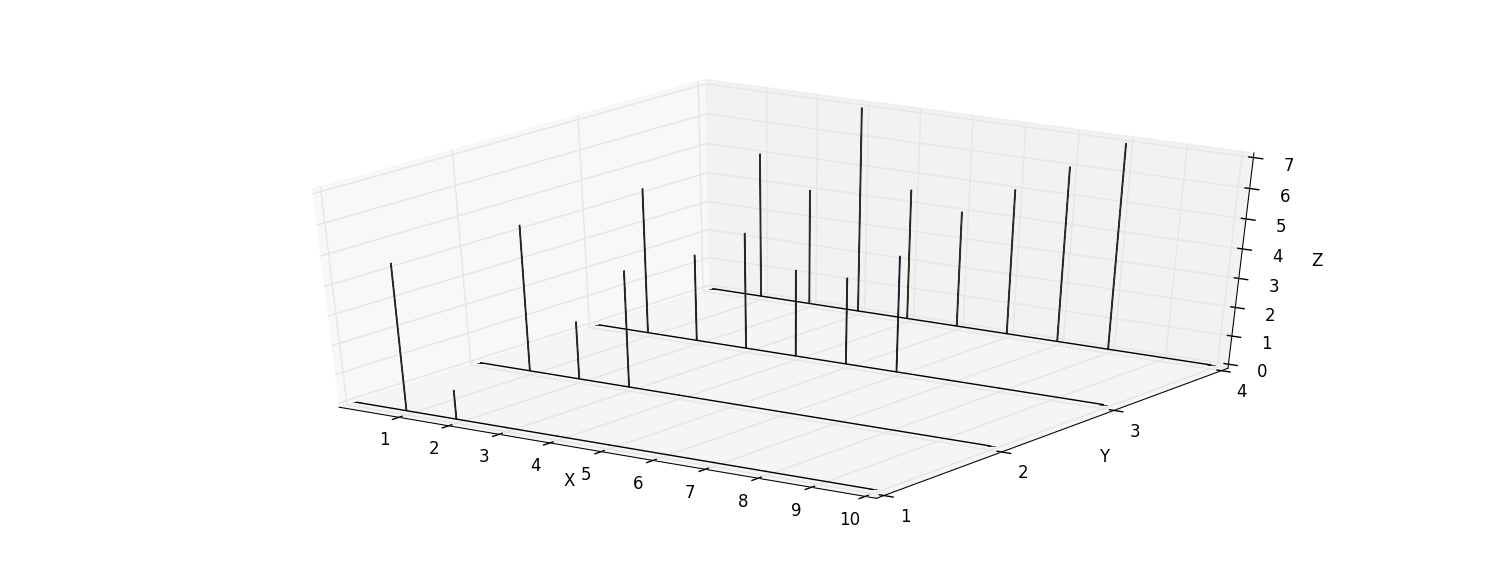
\includegraphics[width=0.9\linewidth]{desalineamientoevolucion}
		 				\caption{evolución de los espectros vibratorio debido al desalineamiento}
		 				\label{fig:desalevolucion} 				
	 				\end{figure}
	 				En la imagen \ref{fig:desalevolucion} se grafican los espectros característicos de la evolución de la falla que produce un desalineamiento donde:
	 				\begin{enumerate}
		 				\item Espectro base (Sin falla, sólo desbalanceo residual)
		 				\item Levemente desalineado
		 				\item Medianamente desalineado
		 				\item Desalineamiento severo 				
		 			\end{enumerate}
	 				Para Desalineamientos severos, la forma del espectro vibratorio es similar al espectro característico del desbalanceo (Sección \ref{sssec:soltura}). La diferencia, o la manera de identificar el desalineamiento es mediante la amplitud en la dirección de la vibración. el tipo mas frecuente de desalineamiento que se encuentra en equipos mecánicos es del tipo combinado (fig \ref{fig:desmixto}) debido a las fuerzas generadas en el mecanismo de acople.
	 				
	 			\subsubsection{Síntomas vibratorios de la soltura mecánica} \label{sssec:soltura}
	 				Se entiende por soltura mecánica a cualquier elemento que se encuentre suelto que influya de manera directa en las vibraciones de la máquina sin distinción sobre si la falla de soltura ocurre en un componente interno o externo del mecanismo. Ejemplos clásicos de soltura en máquinas son:
	 				\begin{itemize}
	 					\item Pernos de sujeción de la máquina a la bases sueltas
	 					\item Juego radial excesivo en rodamientos
	 					\item Grieta en la estructura de la máquina o en el pedestal soporta descansos
	 					\item Rotor suelto en el eje, o con interferencia
	 				\end{itemize}
 					La falla de soltura mecánica en el espectro de frecuencia aparece como un aumento de armónicos de la componente 1X (figura \ref{fig:solturagrafico}) de la máquina, llegando a obtener hasta componentes de 14X dependiendo de la severidad de la soltura.
 					\begin{figure}[H]
 						\centering
 						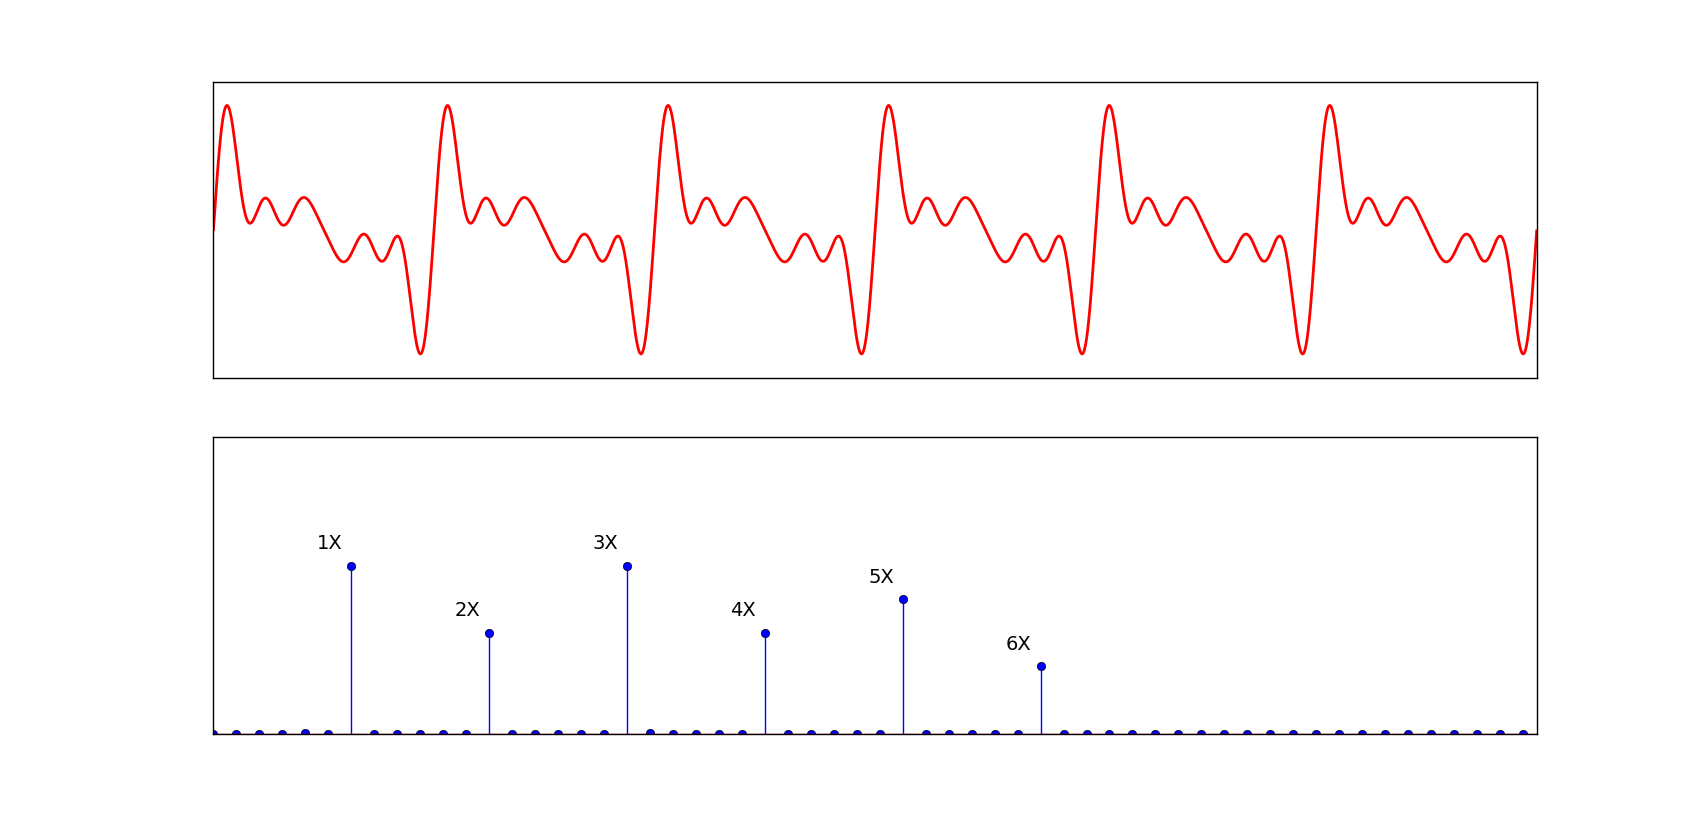
\includegraphics[width=\linewidth]{solturagrafico}
 						\caption{Forma de Onda y FFT característicos de desbalanceo}
 						\label{fig:solturagrafico}
 					\end{figure}
 				\subsubsection{Sintomas Vibratorios en ruedas dentadas}
 					Por Hacer!
 			\subsection{Detección de fallas en rodamientos}
 				El rodamiento es un elemento mecánico utilizado en casi la mayoría de los equipos rotatorios, es por eso que es de vital importancia el análisis o monitoreo de estos componentes en el mantenimiento predictivo.
 				
 				Dentro del ciclo de operación de un rodamiento, aunque este sea montado de manera correcta, con una correcta lubricación, manteniéndolo libre de elementos contaminantes (agentes externos) y calculándolo para una correcta operación se puede decir que el rodamiento estará libre de fallas exceptuando una: la falla por fatiga, la cual no puede ser evitada debido a su tiempo de operación o vida útil. Es por esto que la evolución de la falla de un rodamiento a través del tiempo se puede clasificar en cuatro etapas y es esta clasificación por la cual, la experiencia dice que este tipo de falla ocurre en aproximadamente el $80\%$ de las veces
 				\begin{itemize}
 					\item Etapa 1: El primer indicio de falla en un rodamiento es una grieta a nivel microscópico y sub-superficial, generalmente localizado en el punto de mayor carga del rodamiento (punto de contacto entre el elemento rodante y la pista externa), en esta etapa la detección de la grieta (a nivel microscópico) es imposible de detectar mediante el uso de un acelerómetro y espectros frecuentes, por lo que se deben emplear técnicas mas complejas siendo una de ellas llamada IDF (Incipient Detection Failure) la cual aprovecha la frecuencia natural del acelerómetro para amplificar esta señal de baja amplitud 
 					\item Etapa 2: Una vez que se genero la grieta sub-superficial, esta comenzará a propagarse hacia la superficie produciéndose una pequeña fisura o picadura en el elemento. Esta falla es apenas visible para el ojo humano. Al existir esta picadura, en el momento en el que una bola pasa por esta, se produce un efecto mazo-campana que hace que la bola existe las frecuencias naturales de la pista siendo estas frecuencias de alta frecuencia pero de baja amplitud
 					\item Etapa 3: El paso de las bolas sobre la picadura hace que la picadura aumente en tamaño, haciendo que las componentes de frecuencias en el espectro de velocidad en los elementos del rodamiento (frecuencias cuales son propias de cada elemento del rodamiento -pista externa, interna, jaula o bolas- dependiendo de donde se localiza la picadura [tabla \ref{tab:frecuenciasrodamiento}]) 
 					\item Etapa 4: La falla catastrófica es inminente debido a que la falla ya es de gran magnitud dentro del rodamiento, es de esperar también que el daño ya sea múltiple en los elementos lo que hace que aparezcan mas componentes de falla de los elementos del rodamiento en el espectro y el daño en pistas puede estar distribuida a su largo y no solo concentrado en un punto.
 				\end{itemize}
 				Como se menciono dentro de las etapas de falla de un rodamiento, los impactos generados a partir de un defecto en alguno de los elementos del rodamiento producen una excitación (vibración) cada vez que un elemento rodante hace contacto con la superficie dañada. Esta excitación de los elementos suele ser periódica con relación directa con la velocidad de los elementos rodantes y la geometría del rodamiento.
 				
 				\begin{center}
 					\begin{table}
 						\caption{nomenclatura de las frecuencias características de rodamiento}
 						\label{tab:frecuenciasrodamiento}
	 					\begin{tabular}{| >{\centering\arraybackslash}m{0.4\linewidth} | >{\centering\arraybackslash}m{0.1\linewidth} |>{\centering\arraybackslash}m{0.4\linewidth}| } 		
	 						\hline
	 						Frecuencia característica & \scriptsize{Acrónimo} & Fórmula \\ \hline \hline
	 						Frecuencia de paso de los elementos rodantes sobre la pista externa.
	 						(Ball pass frequency of outer race) & BPFO & $$\frac{RPM\cdot n}{2}\cdot \left (1-\frac{d\cdot\cos{\theta}}{d_{m}}\right )$$ \\ \hline
	 						Frecuencia de paso de los elementos rodantes sobre la pista interna.
	 						(Ball pass frequency of inner race) & BPFI & $$\frac{RPM\cdot n}{2}\cdot\left (1+\frac{d\cdot\cos{\theta}}{d_{m}}\right )$$ \\ \hline
	 						Frecuencia de rotación de la jaula contenedora de las bolas (Fundamental train frequency) & FTF & $$\frac{RPM}{2}\cdot \left (1+\frac{d\cdot\cos{\theta}}{d_{m}}\right )$$ \\ \hline
	 						Frecuencia de giro de los elementos rodantes & BSF & $$\frac{RPM \cdot  d_{m}}{2d}\left[1-\left(\frac{d}{d_{m}}\right)^2 \cos^2(\theta)\right]$$ \\ \hline
	 					\end{tabular}
 					\end{table}					
 				\end{center}
 			\begin{figure}
 				\centering
 				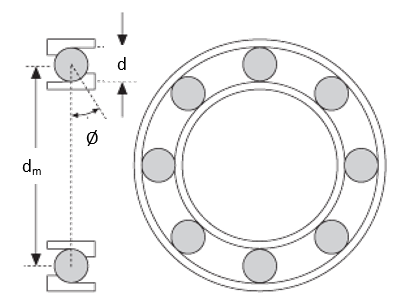
\includegraphics[width=0.6\linewidth]{rodamientoindices}
				\caption{nomenclatura usada en tabla \ref{tab:frecuenciasrodamiento}}
 				\label{fig:rodamientopartes}
 			\end{figure}
 			Donde:
	 		\begin{itemize}
	 			\item $n$: número de elementos rodantes
	 			\item $d$: diámetro de los elementos rodantes
	 			\item $d_{m}$: diámetro entre los centros de los elementos rodantes
	 			\item $RPM$: revoluciones por minuto de giro del rodamiento
	 		\end{itemize}
	 	La señal que se obtiene al medir un rodamiento poseen un comportamiento especial dependiendo del elemento que presente la falla, en especial aquellos rodantes (pista interna -En la mayoría de las aplicaciones en la cual gira-,elementos rodantes), pues estos están constantemente pasando y saliendo por la zona de alta carga, originándose una señal modulada en amplitud, pues el elemento al chocar en la zona de alta carga tendrá una respuesta mayor en amplitud que cuando esta misma pase por la zona de mínima carga.
 		\begin{figure}
			\centering
			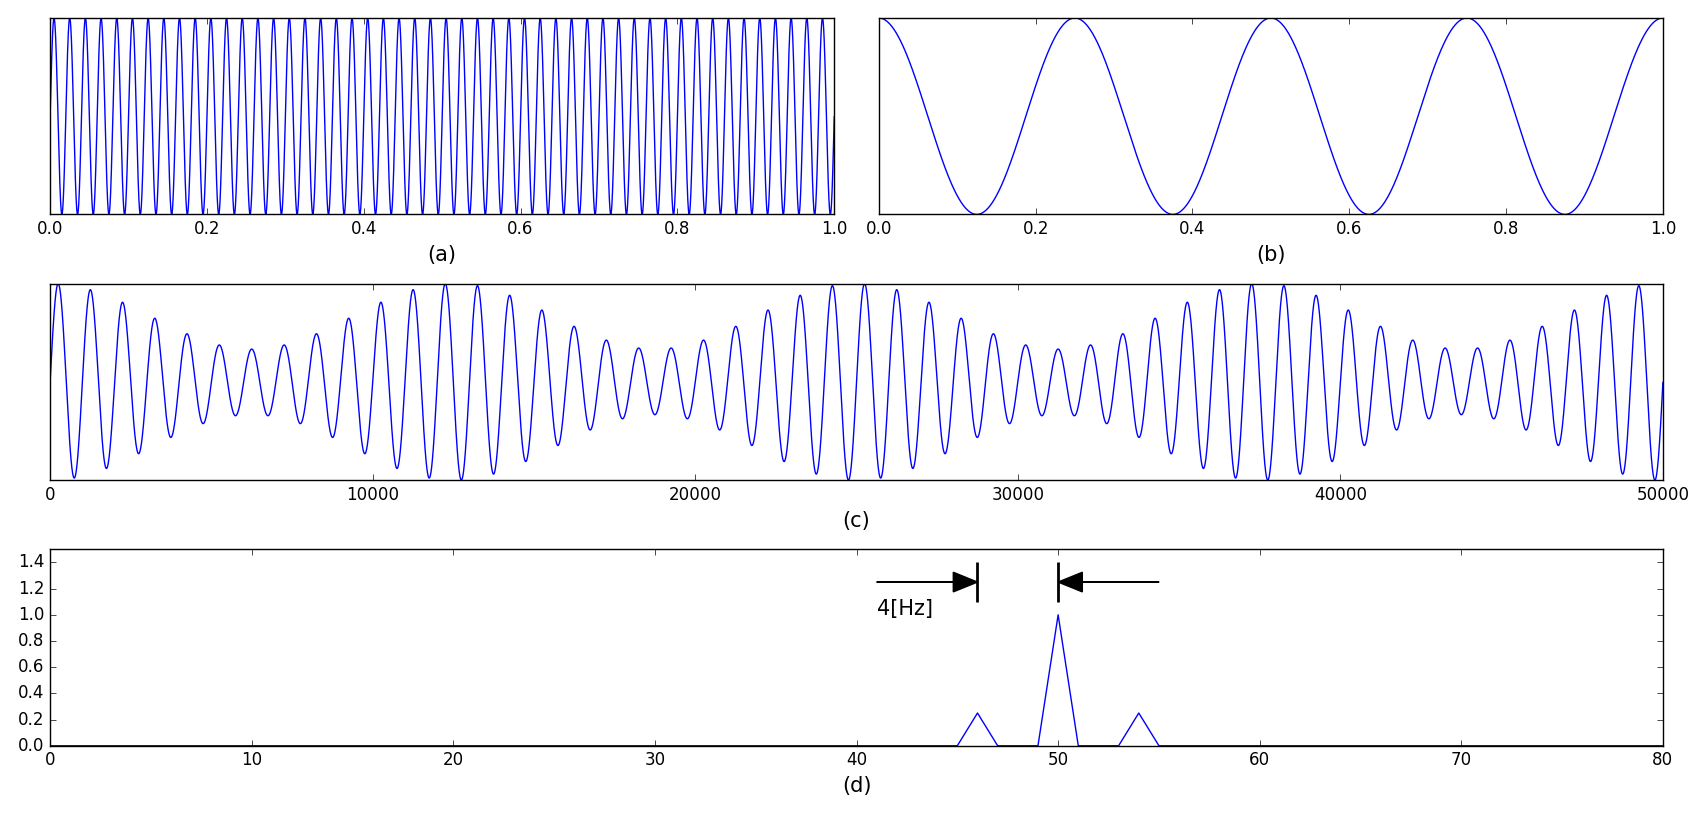
\includegraphics[width=\linewidth]{modulacion}
			\caption{Ejemplo de señal modulada en amplitud}
			\label{fig:modulacion}
		\end{figure}
		
		\subsubsection{Señales moduladas en amplitud}
			La modulación en amplitud consiste en una interacción particular entre dos señales diferentes, donde la amplitud de una señal varía en relación a la señal transmitida o la señal modulada, es decir, donde por lo general la frecuencia de la onda portadora es mayor a la onda modulada, matemáticamente se tiene la siguiente relación para la modulación en amplitud: 
			
			Una señal portadora de forma trigonométrica:\\
			
			\begin{equation}
				p(t) = A \cdot \sin \left(2 \pi f_{p}t \right)			
			\end{equation}
			
			Una señal la cual sera modulada por la señal portadora: 
			
			\begin{equation}
				m(t)= M \cdot \sin \left(2 \pi f_{m} t \right) 
			\end{equation}
			
			Finalmente, la modulación con la señal portadora se expresa como: 
			
			\begin{equation}
				y(t)=\left[m(t)+1\right ]\cdot p(t)				
			\end{equation}
			donde: 
			
			\begin{itemize}
				\item $p(t)$: Onda portadora
				\item $m(t)$: Onda a montar
				\item $A$ y $M$: Amplitud de cada onda
				\item $f_{p}$ y $f_{m}$: Frecuencia de cada onda
				\item $y(t)$: señal modulada en amplitud
			\end{itemize}
			
			Un ejemplo de modulación en amplitud se puede apreciar en la imagen \ref{fig:modulacion} donde se tienen dos señales, (a) con una frecuencia de $50[Hz]$ y (b) con una frecuencia correspondiente de $4[Hz]$, en (d) se puede ver la forma característica de la modulación en amplitud que consiste en una frecuencia central, correspondiente a la señal portadora y dos frecuencias a ambos lados correspondientes a la onda montada, la distancia entre estas frecuencias es equivalente a la de la onda montada. En la práctica las modulaciones en amplitud suelen contar con mayor numero de lineas laterales debido a los armónicos de la señal.\\
			
			Estas señales moduladas en fallas en rodamientos, la señal moduladora contiene la información acerca de las fallas características es que existen técnicas (procesamiento de la señal) para extraer las frecuencias de interés Una de estas herramientas es calcular hacer uso de la señal analítica (señal que se caracteriza por no contener frecuencias negativas) para así calcular la envolvente de la señal usando la transformada de Hilbert, la cual se define, para una señal arbitraria $f(t)$ como \cite{Boashash1992}:
			\begin{equation}
				H \{f(t)\} = p.v \cdot \int_{-\infty}^{\infty} \frac{f(t-\tau)}{\pi \tau} d\tau
			\end{equation}
			donde $p.v$ corresponde al valor inicial de Cauchy. Una señal con valores reales, como las medidas en vibraciones puede ser representada de forma analítica de la siguiente manera:\\
			\begin{equation}
				s_{a}=s(t)+j \cdot H[s(t)]
			\end{equation}
			de esta manera, analíticamente, la señal esta representada de manera compleja, por lo que puede expresarse de manera compleja de la forma:\\
			\begin{equation}
				s_{a}(t) = s_{m}(t) \cdot e^{j\phi (t)}			
			\end{equation}
			donde $|s_{a}|$ corresponde a la amplitud instantánea y $\arg\left (|s_{a}(t)|\right )=\phi(t)$ a la fase. Dos ejemplos de envolventes mediante la transformada de Hilbert pueden verse en la imagen \ref{fig:hilbert1} y \ref{fig:hilbert2}
			\begin{figure}[H]
				\centering
				\begin{subfigure}[b]{\linewidth}
					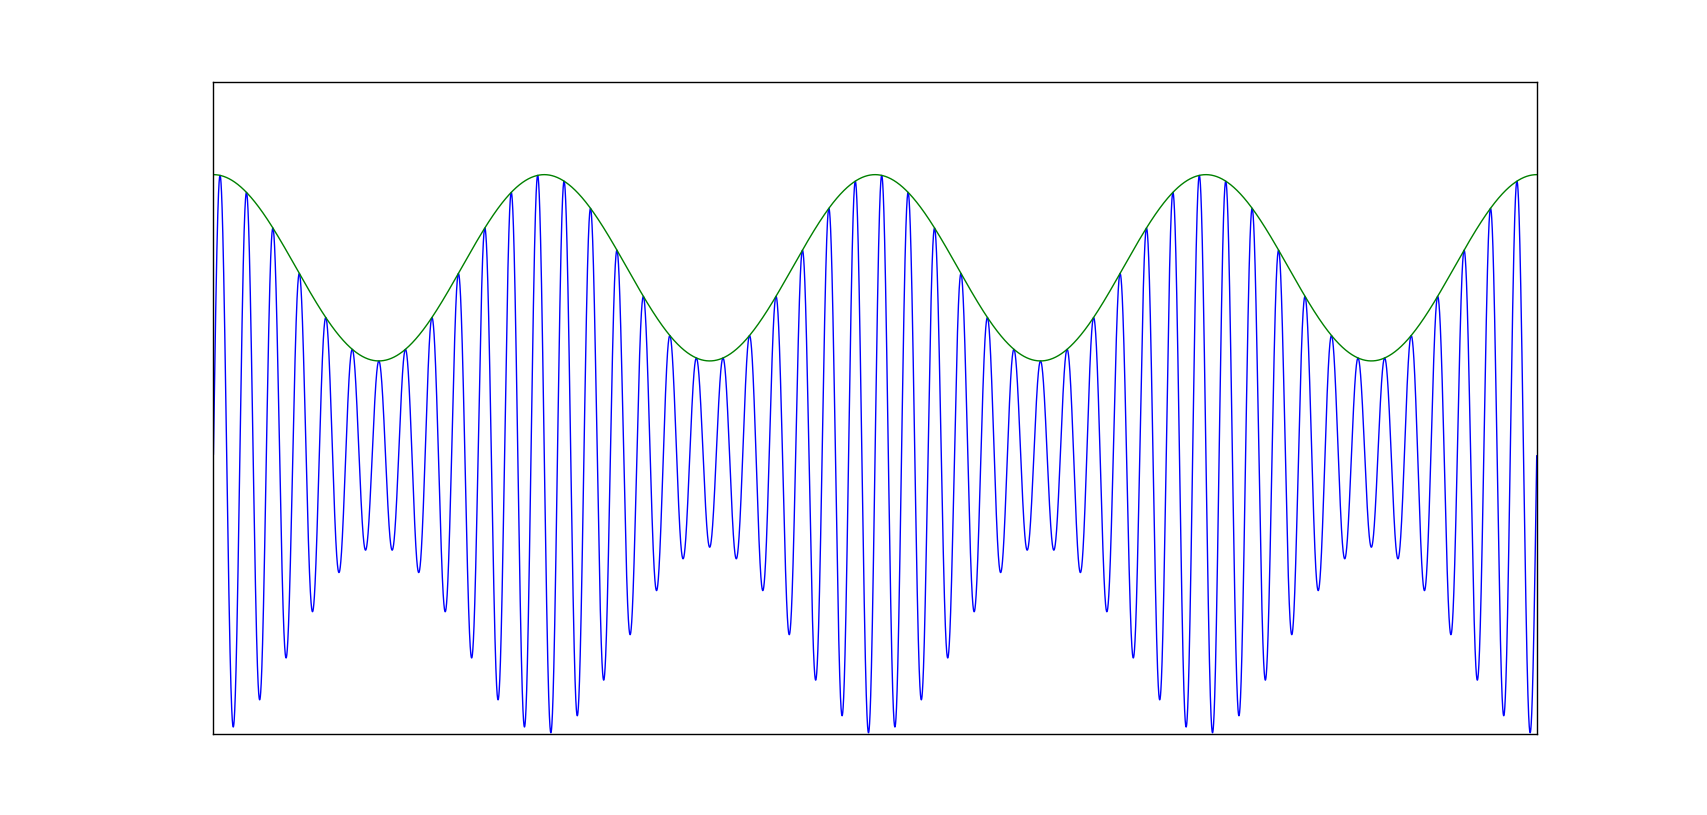
\includegraphics[width=0.9\linewidth]{hilbert1}
					\caption{Envolvente de señal pura}
					\label{fig:hilbert1}
				\end{subfigure}
				\begin{subfigure}[b]{\linewidth}
					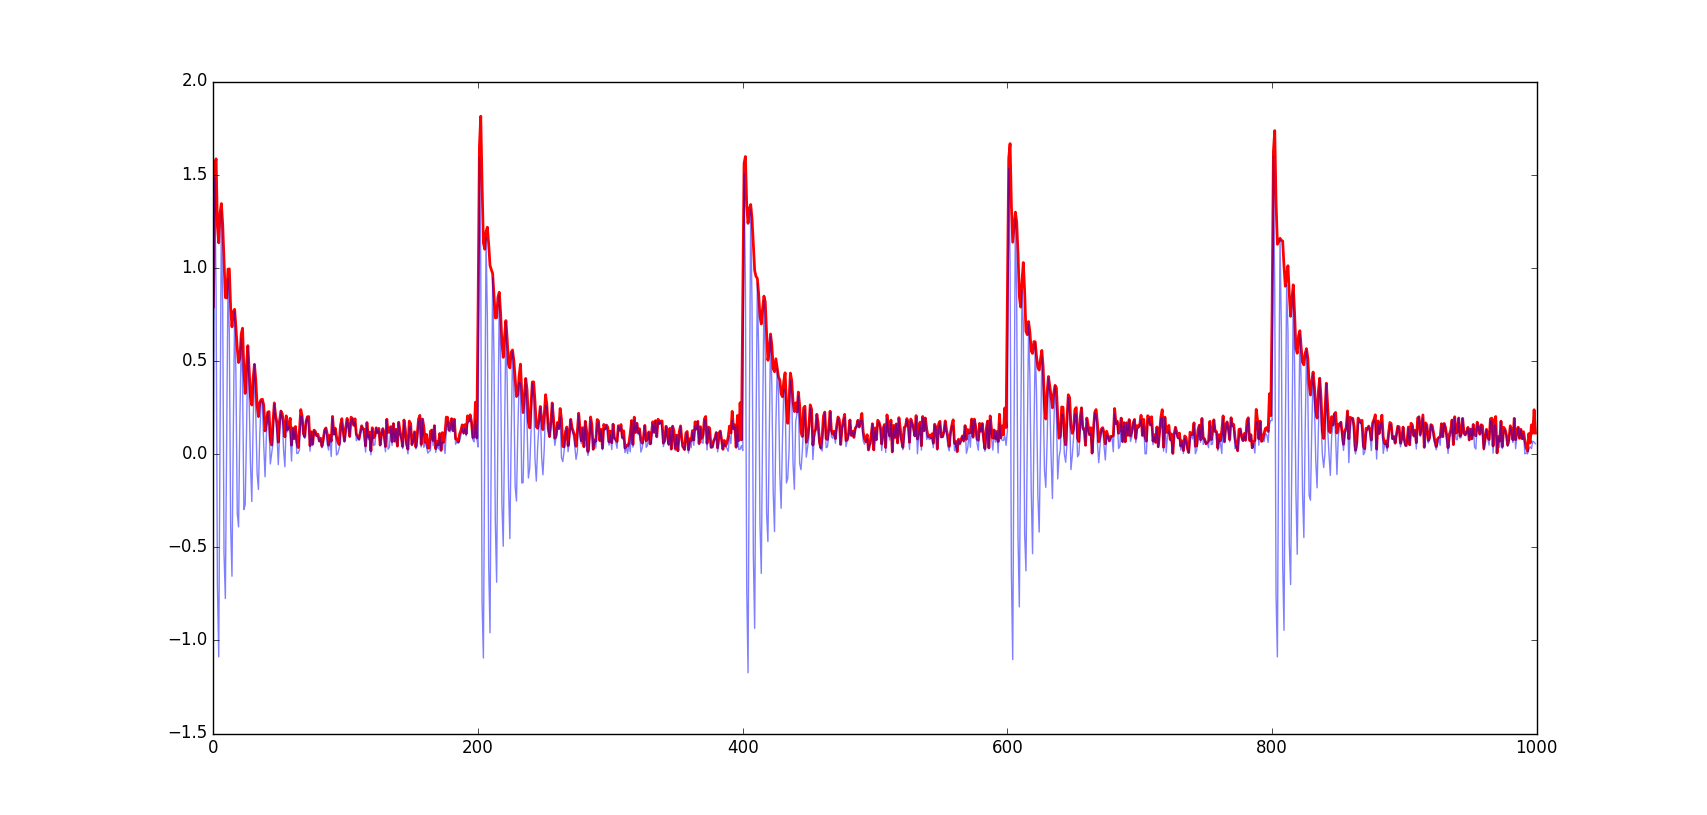
\includegraphics[width=0.9\linewidth]{hilbert2}
					\caption{Envolvente de una señal impulsiva con ruido gaussiano}
					\label{fig:hilbert2}
				\end{subfigure}
				\caption{Ejemplos de envolvente mediante transformación de Hilbert}
				\label{fig:hilbert}						
			\end{figure}
		El procedimiento para aislar la señal de interés consiste en los siguientes pasos:
		\begin{enumerate}
			\item {Calcular FFT de la señal a analizar}
			\item Seleccionar filtro pasa banda procurando dejar la zona donde se ve comportamiento de modulación en amplitud
			\item En el caso de querer estudiar severidad, debe aplicarse una ganancia a la señal filtrada
			\item Calcular la señal analítica de la señal mediante la transformada de Hilbert para calcular envolvente
			\item Calcular FFT de la señal envolvente
			\item Corroborar si aparecen tonos de rodamientos (BPFO,BPFI...) 
		\end{enumerate}
		
		\section{Análisis en equipos a baja velocidad}
			\subsection{Desafío a bajas revoluciones}
			    Predecir la presencia de fallas en equipos que operan a bajas revoluciones utilizando las técnicas de espectros resulta ser una tarea difícil de llevar a cabo, principalmente debido a que el giro de estos equipos por lo general no son lo suficientemente rápidos como para generar las fuerzas dinámicas significantes como para manifestarse en la forma de onda del fenómeno que se esta midiendo por lo que esta señal, en caso de no ser nula, resulta ser de baja amplitud pasando estas desapercibidas por el nivel de ruido del entorno. Las máquinas consideradas de bajas revoluciones son aquellas que giran entre 6 y 300 ciclos por minuto \cite{robinsonjc}			
			\subsection{Estado actual de técnicas a bajas revoluciones}
			    Debido a que en este tipo de máquinas las fuerzas dinámicas suelen ser bajas es que las manifestaciones clásicas de fallas suelen no aparecer exceptuando fallas localizadas como lo son por ejemplo fallas en rodamientos que generan señales con características no estacionarias y transcientes (Señales que empiezan y terminan en cero en un tiempo finito \cite{dlinonstationary}). A continuación se resumen tres técnicas usadas en el análisis a baja velocidad que tienen como objetivo el análisis de fallas en rodamientos:
			    \subsubsection{Análisis de forma de Onda}
			        Como el efecto o falla de rodamiento es de tipo localizado, cada vez que un elemento rodante pasa por la falla, se produce un impacto que produce una vibración no estacionaria. El análisis de la forma de onda de aceleración permite identificar los impactos producidos por el paso de los elementos rodantes. Un ejemplo de este análisis esta propuesto en \textit{análisis de vibraciones aplicados a las maquinas rotatorias de baja velocidad} \cite{pedrosaav}
			        \begin{figure}
			            \centering
			            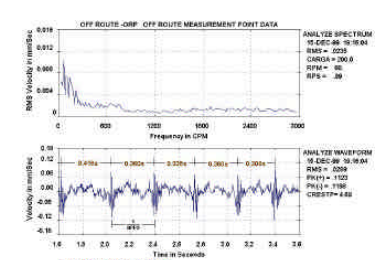
\includegraphics{formaondasaavedra}
			            \caption{Espectro y forma de onda de rodamiento con pista externa defectuosa y velocidad variable}
			            \label{fig:rodsaav}
			        \end{figure}
			        En la figura \ref{fig:rodsaav} se muestra tanto la forma de onda como el espectro de frecuencia medido en un agitador que presenta fallas en la pista externa del rodamiento, la velocidad nominal del equipo son 60 rpm. Si se analiza el espectro tomado, no se puede observar la componente de frecuencia correspondiente al rodamiento. Sin embargo, si se analiza la serie de tiempo, se pueden notar impactos a un tiempo aproximadamente el inverso del tono de rodamiento BPFO confirmando una existencia de falla en rodamiento
			     \subsubsection{Análisis Espectral promediando en frecuencia}
			        Esta técnica se basa en promediar diferentes mediciones realizadas de igual manera con el fin de promediar los espectros, obviando así la diferencia de fase que se pueda presentar entre mediciones. Esto hace que tanto el ruido electrónico como señales del entorno (aleatorias) disminuyan manteniendo en alto aquellas que no varían de manera aleatoria (señal de interés) esto mejora la relación señal/ruido de las mediciones. Un factor importante es que para esta técnica también se necesita una alta resolución en frecuencia (numero de lineas). Esto aumentando el tiempo de adquisición de la señal a analizar.
			        En la figura \ref{fig:fftpromedio} puede verse como mejora el espectro al aumentar el numero de promedios y el numero de lineas (Fuente: \cite{pedrosaav}).
        			\begin{figure}[H]
        				\centering
        				\begin{subfigure}[b]{\linewidth}
        				    \centering
        					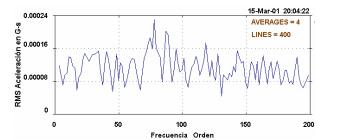
\includegraphics{fftpromedio1}
        					\caption{Espectro con 4 promedios y 400 líneas de resolución}
        					\label{fig:fftpromedio1}
        				\end{subfigure}
        				\begin{subfigure}[b]{\linewidth}
        				    \centering
        					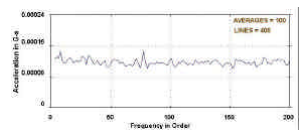
\includegraphics{fftpromedio2}
        					\caption{Espectro con 100 promedios y 400 lineas de resolución}
        					\label{fig:fftpromedio2}
        				\end{subfigure}
        				\begin{subfigure}[b]{\linewidth}
        				    \centering
        					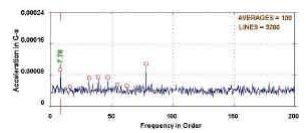
\includegraphics{fftpromedio3}
        					\caption{Espectro con 100 promedios y 3200 lineas de resolución}
        					\label{fig:fftpromedio3}
        				\end{subfigure}
        				\caption{Ejemplo de espectros para diferente configuración de promedios y resolución}
        				\label{fig:fftpromedio}
        			\end{figure}	
        		\subsubsection{Curtosis correlacionada y curtogramas}
        		    Este último método es una herramienta estadística para analizar ondas no estacionarias (como rodamientos) debido a que es capaz de indicar la presencia de series transientes y las frecuencias locales en el dominio de frecuencias. La idea general es la de modelar la señal como una suma lineal entre una señal transiente (débil) y ruido, es decir:
        		    \begin{equation}  		         		        
        		        Y(t)=X(t)+N(t)
        		    \end{equation}
        		    en el cual X(t) es la señal transiente y N(t) es ruido. 
        		    
        		    Una manera de analizar este tipo de señal es considerando indicadores estadísticos sensibles a la señal con series de picos (abrupta). Un indicador útil es la curtosis la cual adopta valores altos cuando la señal es del tipo X(t) (figura \ref{fig:curtosiss}) y idealmente cero cuando se tiene sonido de fondo N(t).
        		    \begin{figure}
        		        \centering
        		        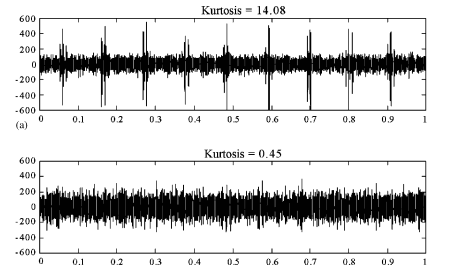
\includegraphics{kurtosis}
        		        \caption{curtosis para dos tipos de señales}
        		        \label{fig:curtosiss}
        		    \end{figure}
        		    La curtosis espectral (SK) presentada por Antoni propone la aplicación de la curtosis localmente para diferentes bandas de frecuencias, ayudando así a evitar que las vibraciones de señales fuertes, repartidas en un rango largo de frecuencias, intervengan con la señal de interés, este proceso de filtrado se le conoce como curtosis espectral la cual se calcula mediante \cite{antoni2006spectral}:
        		     \begin{equation}
        		        K_x(f)= \frac{\langle |H(n,f)|^4 \rangle}{\langle |H(n,f)|^2 \rangle^2}-2
        		    \end{equation}
        		    donde:
        		    \begin{equation}        		        
        		        \langle f(n) \rangle = \lim_{N\to\infty} \frac{1}{N} \sum_{N} f(n)
        		    \end{equation}
        		    y $|H(t,f)|$ representa la envolvente compleja de la señal x(t) a la frecuencia f.
        		    
        		    Las propiedades principales de la SK son:
        		    \begin{itemize}
        		        \item la SK the un proceso estacionario es una constante en función de la frecuencia
        		        \item la SK de un proceso Gaussiano Estacionario es 0
        		        \item en la presencia de ruido ($N(t)$), la SK del proceso no estacionario x(n) es:
        		    \end{itemize}
        		    \begin{equation}
        		        K_y(f)=\frac{K_x(f)}{\left[1+\rho(f)\right]^2}
        		    \end{equation}
        		    donde:
        		    \begin{enumerate}
        		        \item $K_x(f)$: SK de señal X(t)
        		        \item $K_y(f)$: SK de señal Y(t)
        		        \item $\rho(f)$: relación ruido-señal
        		    \end{enumerate}
        		    Esta fórmula indica que si la relación señal-ruido es alta, $K_x(f)$ tiende a ser igual a $K_y(f)$ y $K_y$ tiende a  0 cuando la relación es baja.  
        		    las propiedades (1) y (2) muestran la habilidad de la SK para detectar, caracterizar y localizar en frecuencia la parecencia de señales no estacionarias escondidas en los datos.
    			    
    			    SK se ve afectada por el largo de la ventana elegida. Es por eso que Antoni \cite{antoni2006spectral} propone el uso de la transformada de Fourier corta en tiempo para calcular SK con diferentes tamaños de ventana y poder seleccionar el ancho de banda en frecuencia donde la curtosis es mayor. Esta técnica introduce el concepto de curtogramas, el cual es una representación gráfica de SK para diferentes anchos de banda y centradas a diferentes frecuencias, herramienta que debido a su rápido calculo está siendo aplicado en el análisis de falla en rodamiento actualmente.
    			    \begin{figure}[H]
    			        \centering
    			        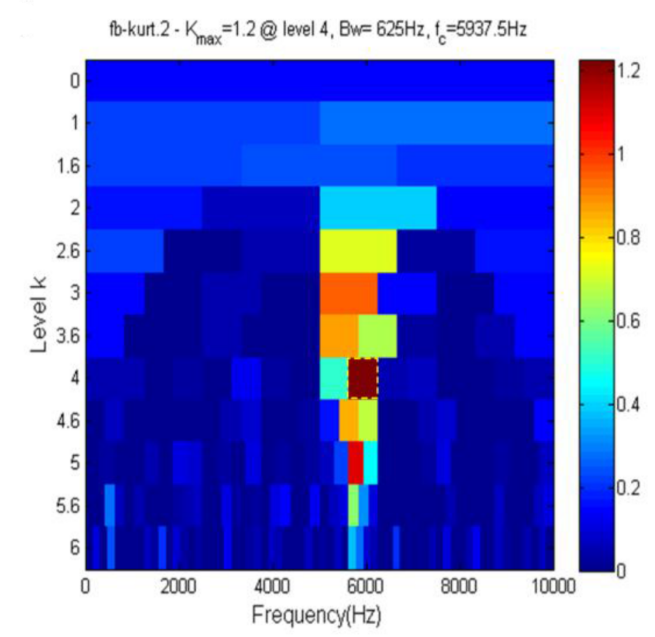
\includegraphics[width=0.5\linewidth]{ejemplokurtograma}
    			        \caption{Ejemplo curtograma}
    			        \label{fig:curtogramaejemplo}
    			    \end{figure}
    			En la figura \ref{fig:curtogramaejemplo} se observa un ejemplo de curtograma para una señal, se puede observar que el mayor valor de curtosis se encuentra en torno a los $6000[Hz]$ con un ancho de frecuencia de $\Delta f= 1250 [Hz] $, el cual se encuentra en el nivel $k=4$. Estos datos permiten la elección de un filtro para demodular el tipo de señal buscada, centrando el filtro en $f_c$ con un ancho de filtro de $\Delta f$.
    			Hoy en día existen varios trabajos relacionados con encontrar fallas en rodamientos empleando la técnica de los curtogramas, a continuación se presenta uno de ellos tomado de \cite{Konstantinos2016} en el cual se detectan fallas en rodamientos en un motor lubricante dentro de un barco.
    			
    			El proceso de análisis de la señal se muesta en la tabla \ref{fig:procesokurtograma}
    			\begin{figure}
    			    \centering
    			    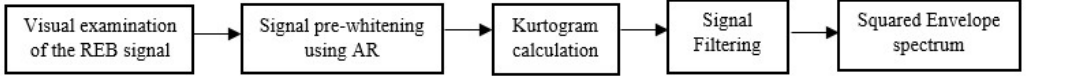
\includegraphics[width=0.7\linewidth]{procesokurtograma}
    			    \caption{Pasos para demodulacion de señal}
    			    \label{fig:procesokurtograma}
    			\end{figure}
    			
    			El autor del trabajo analiza la señal a una tasa de muestreo de $44.1 [kHz]$ sobre un rodamiento modelo 6222 SKF el cual presenta fallas en su pista externa, por lo que es de esperar componentes en el espectro correspondientes al tono de rodamiento BPFO (4.07X)
    			la serie de tiempo junto con el espectro se muestran en la figura \ref{fig:ejkurtograma}
    			\begin{figure}
    			    \centering
    			    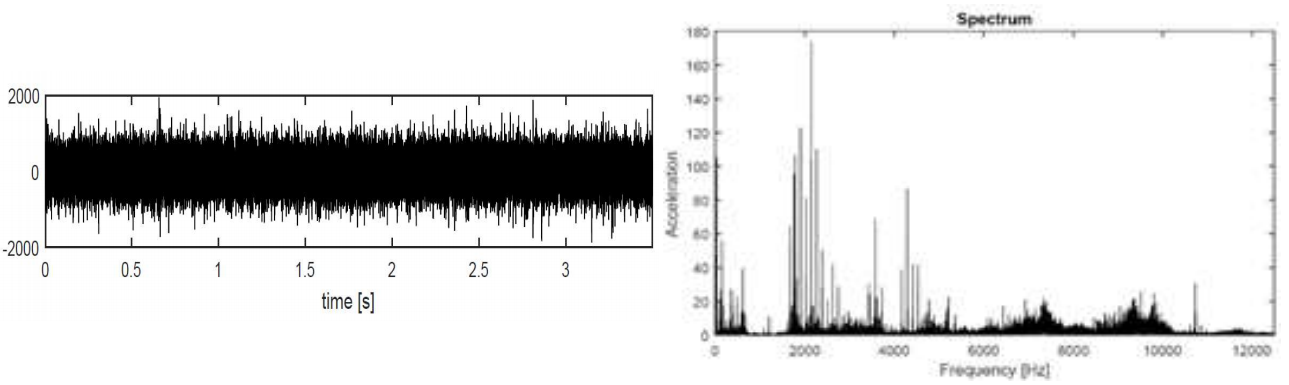
\includegraphics[width=0.75\linewidth]{ejkurtograma}
    			    \caption{Serie de tiempo (izquierda) y su espectro (derecha}
    			    \label{fig:ejkurtograma}
    			\end{figure}
    			Un pre-blanqueado de la señal y una posterior demodulación de la señal muestran resultados claros de una falla en la pista externa teniendo como resultado lo expuesto en la figura \ref{fig:ejkurtograma2}
    			\begin{figure}[H]
    			    \centering
    			    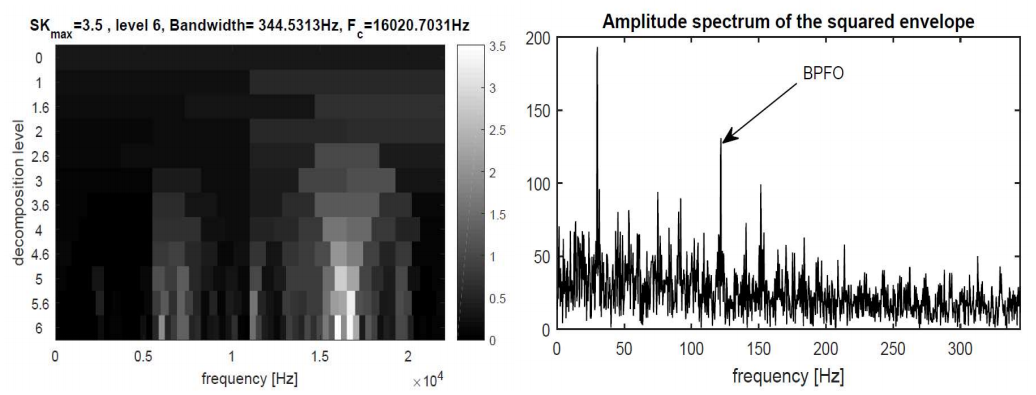
\includegraphics[width=0.75\linewidth]{ejkurtograma2}
    			    \caption{Aplicación curtograma (izquierda) y su demodulación (derecha)}
    			    \label{fig:ejkurtograma2}
    			\end{figure}
    			Del curtograma se ve que la frecuencia central de 16020 [Hz], con un ancho de frecuencias de 344.53 [Hz] posee el mayor valor de curtosis.